\documentclass[../../../main]{subfiles}
\begin{document}

\section{考察}\label{sec:consideration}

\subsection{P制御とPD制御}

図\ref{fig:oscilloscope-each}より
各$P$、$D$ごとに波形を重ねて書いたものを図\ref{fig:oscilloscope-grouped-p}、\ref{fig:oscilloscope-grouped-d}に示す。
\begin{figure}
	\centering
	\begin{subfigure}{0.48\columnwidth}
		\centering
		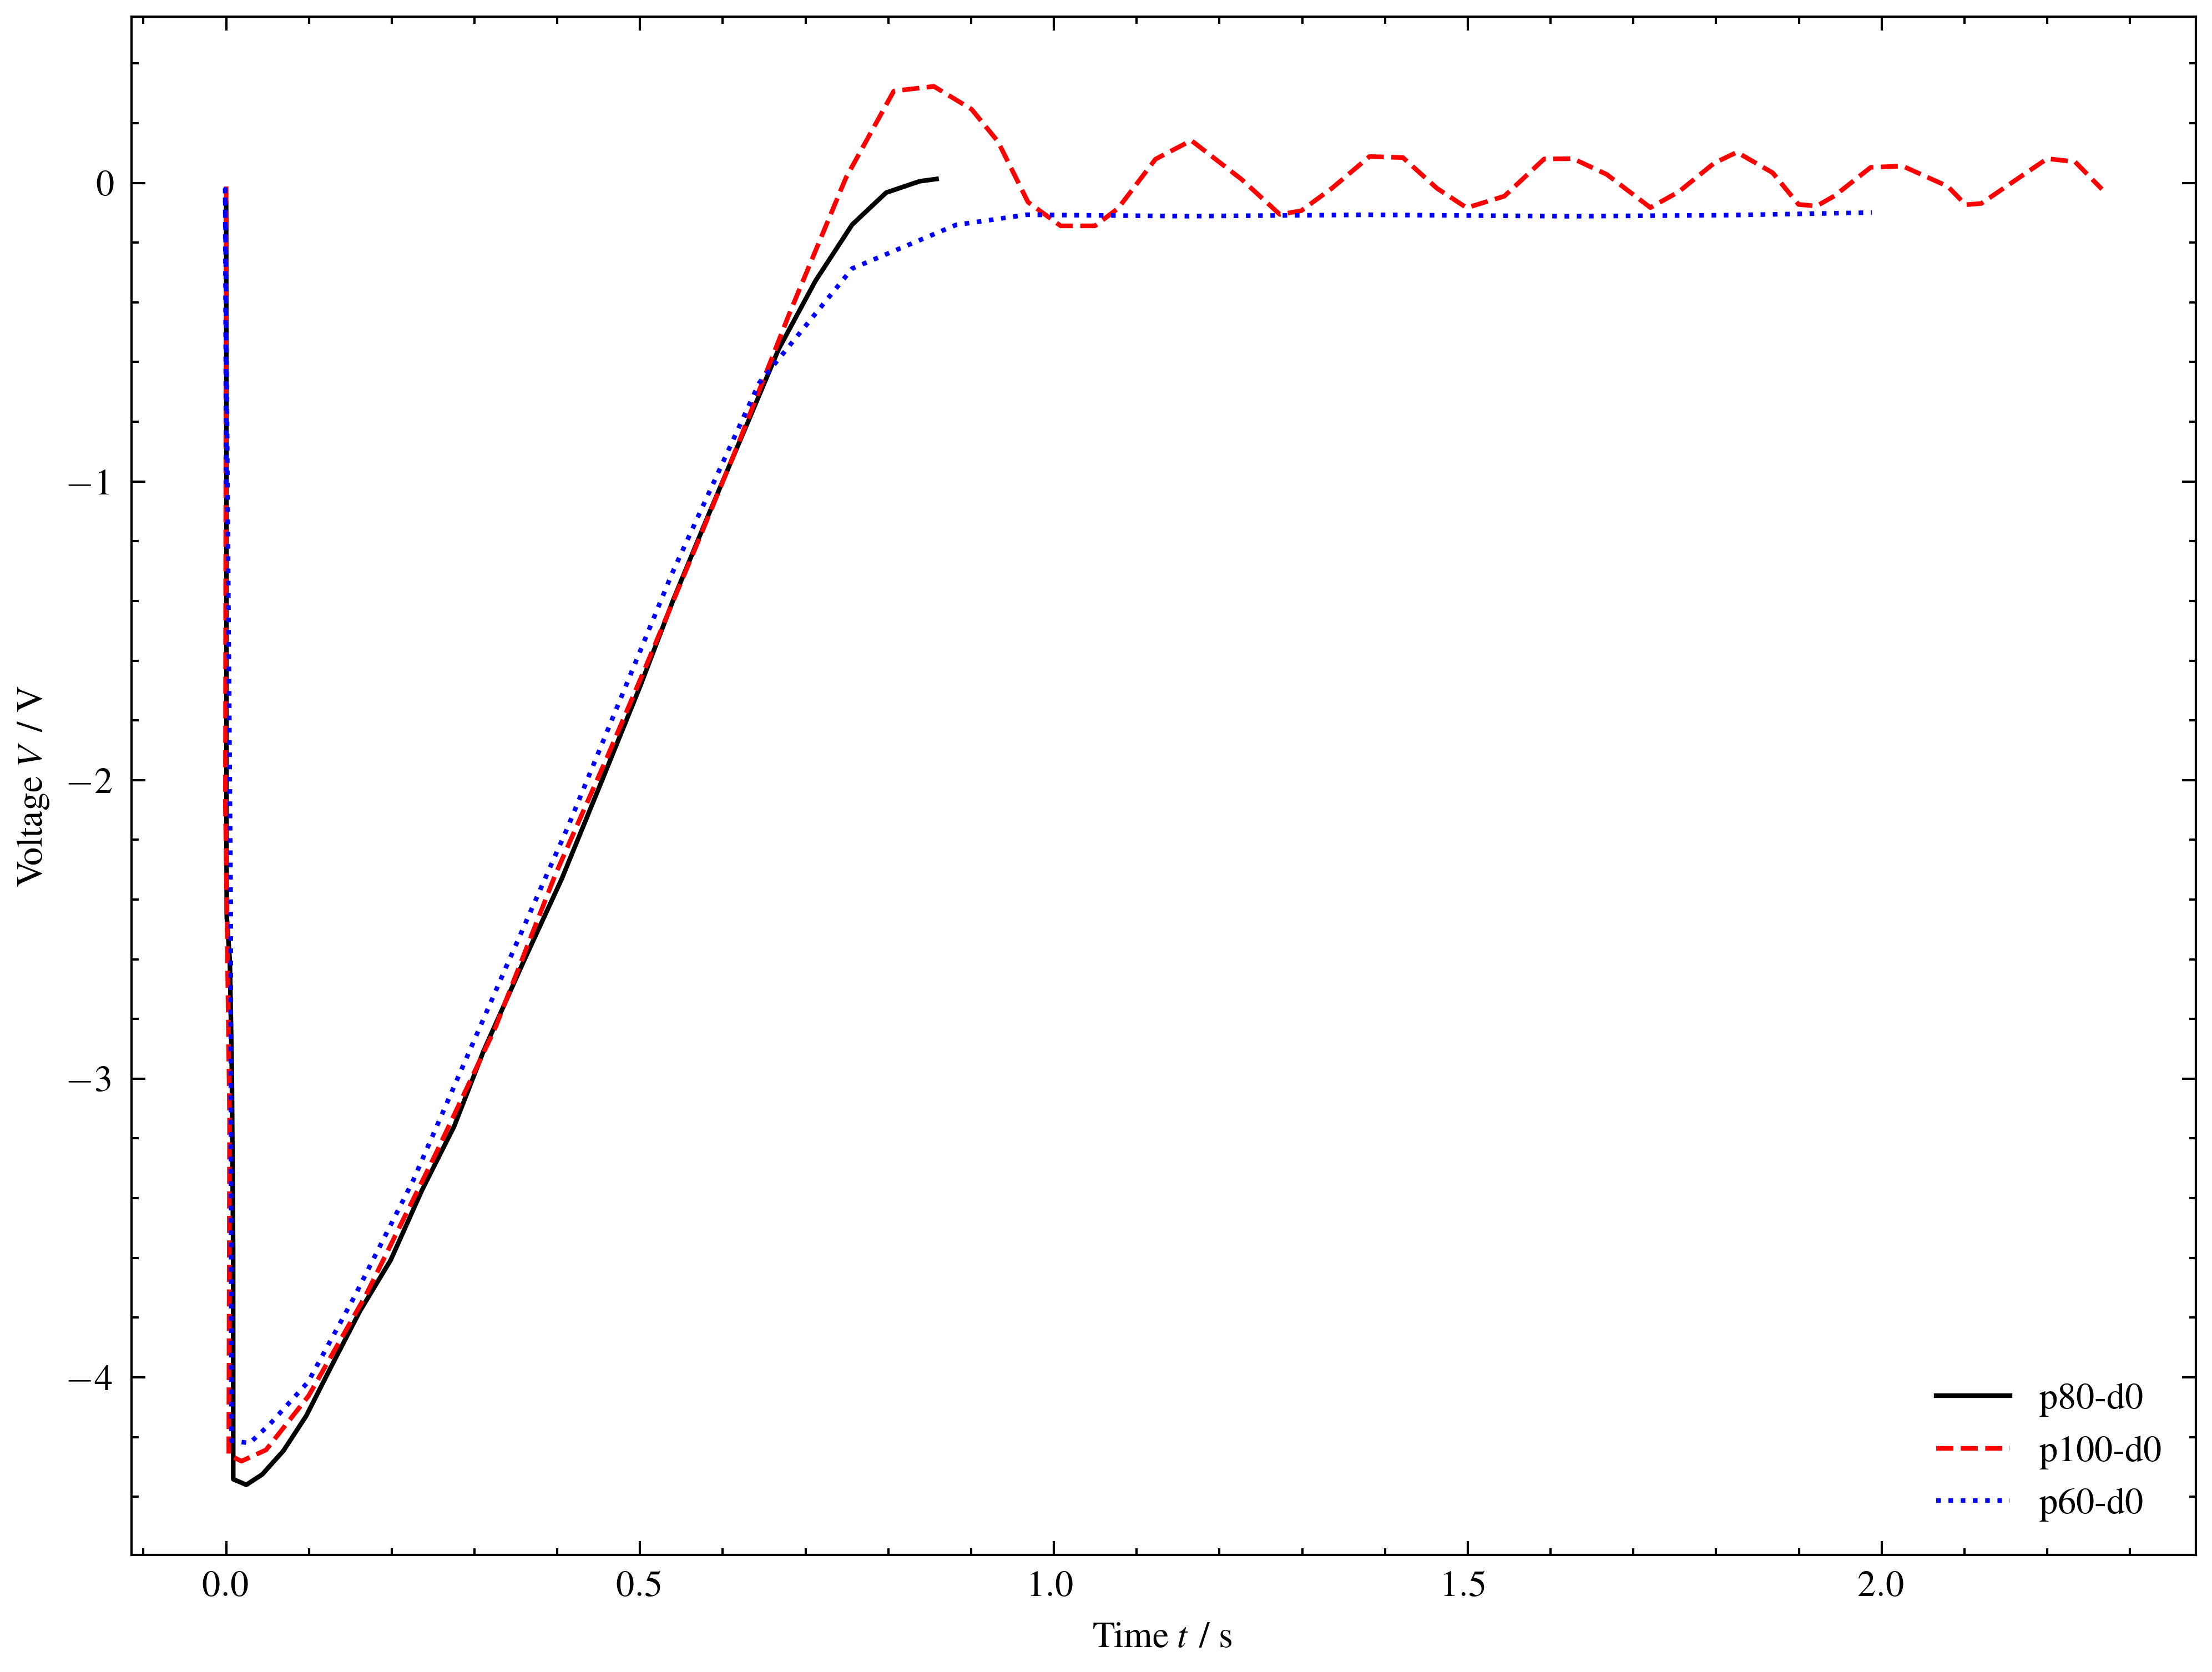
\includegraphics[width=0.8\linewidth]{src/figures/oscilloscope-grouped/d-0.png}
		\subcaption{$D = 0$}
	\end{subfigure}
	\begin{subfigure}{0.48\columnwidth}
		\centering
		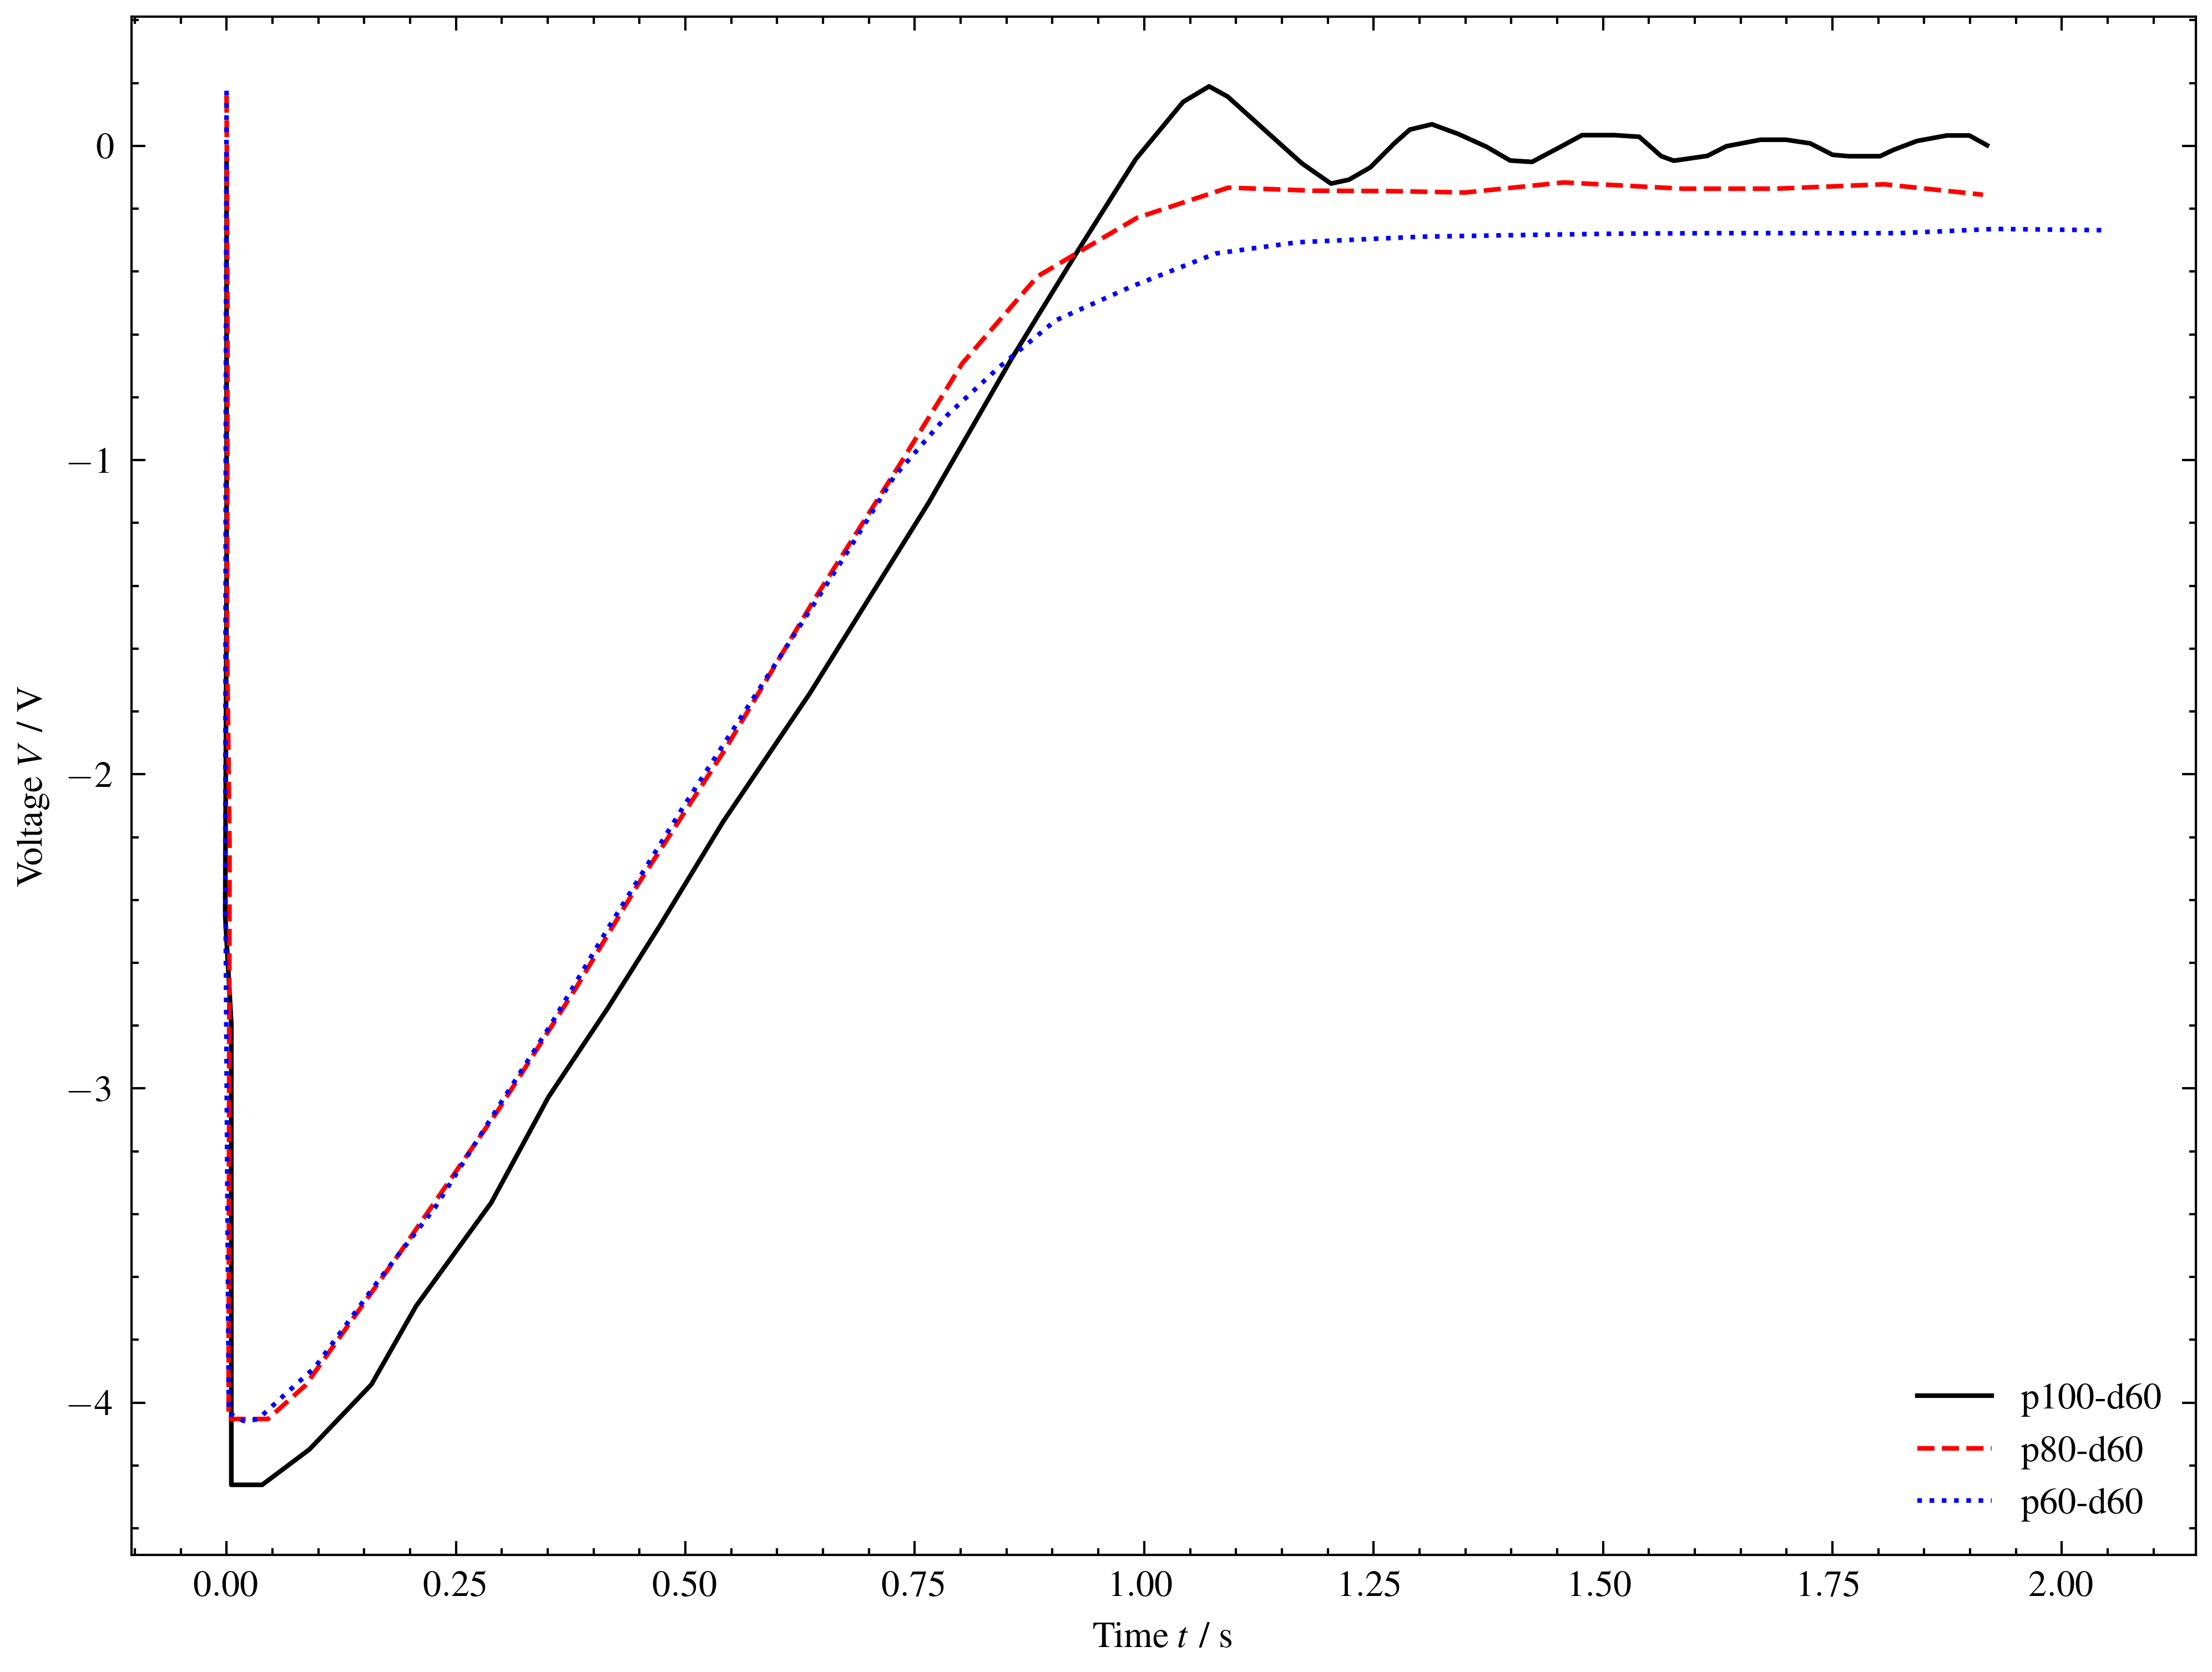
\includegraphics[width=0.8\linewidth]{src/figures/oscilloscope-grouped/d-60.png}
		\subcaption{$D = 60$}
	\end{subfigure}
	\begin{subfigure}{0.48\columnwidth}
		\centering
		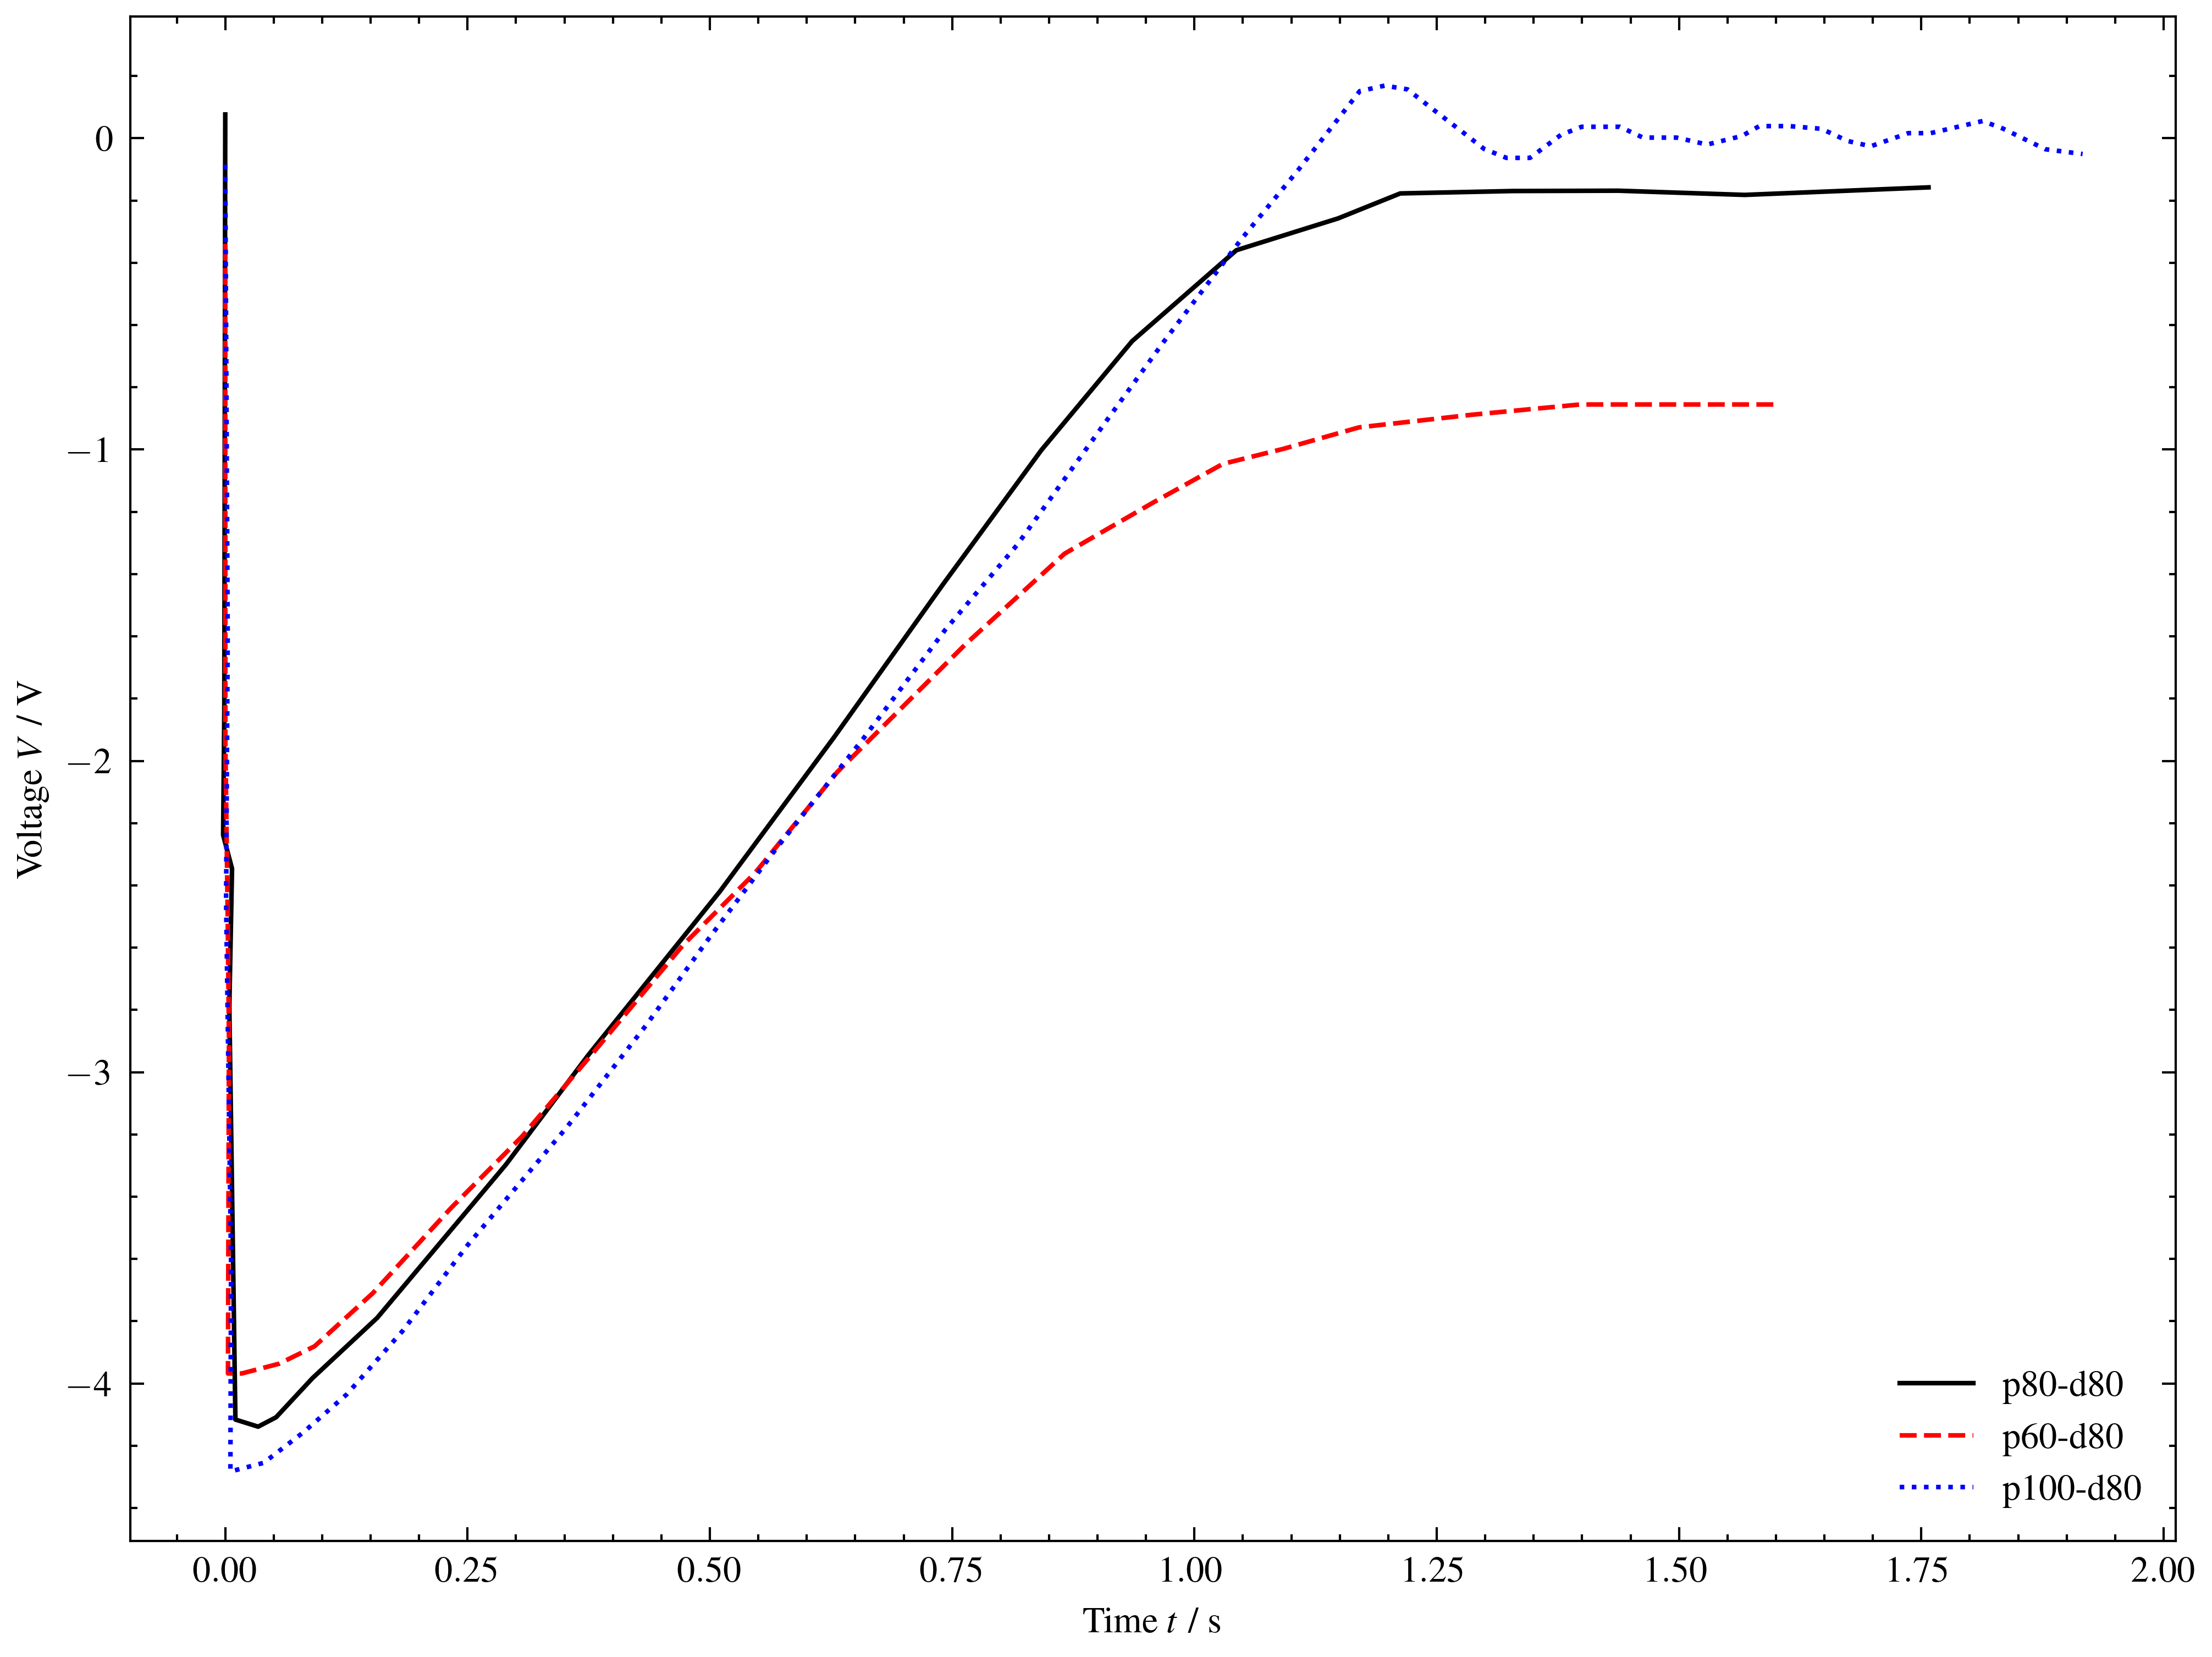
\includegraphics[width=0.8\linewidth]{src/figures/oscilloscope-grouped/d-80.png}
		\subcaption{$D = 80$}
	\end{subfigure}
	\begin{subfigure}{0.48\columnwidth}
		\centering
		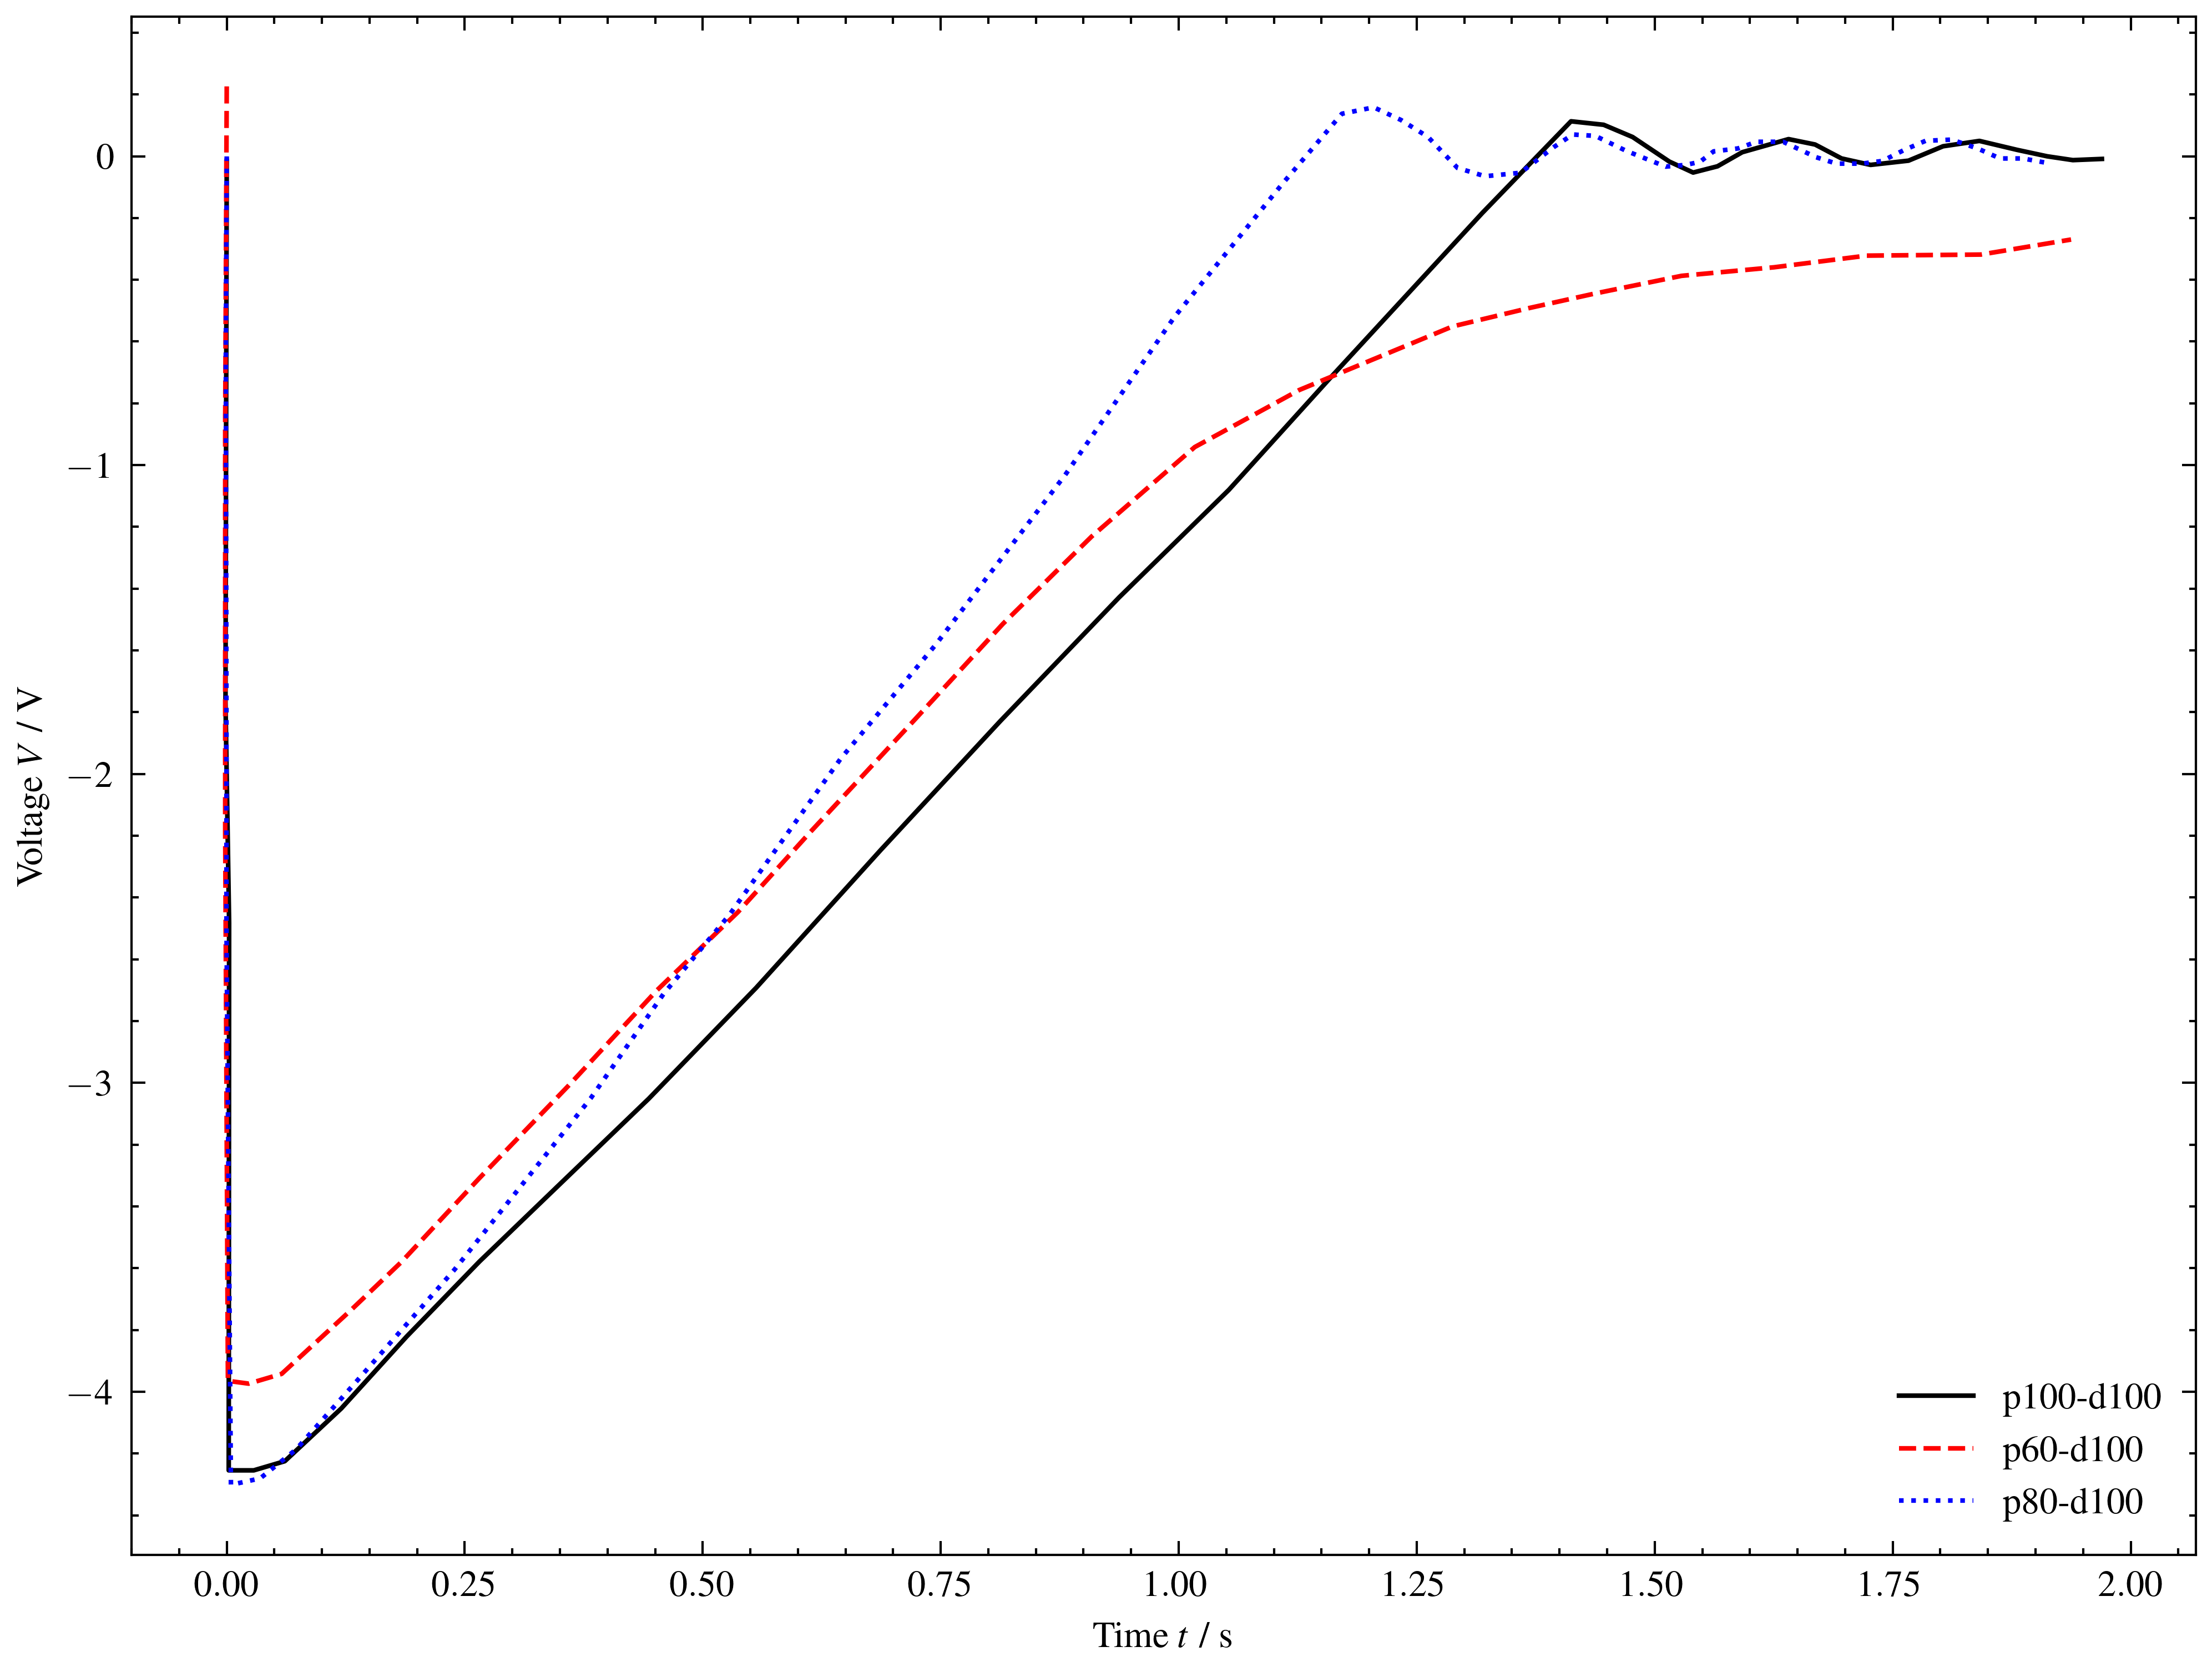
\includegraphics[width=0.8\linewidth]{src/figures/oscilloscope-grouped/d-100.png}
		\subcaption{$D = 100$}
	\end{subfigure}
	\caption{ある$D$に対する$P$を変化させたときの波形}\label{fig:oscilloscope-grouped-d}
\end{figure}

\begin{figure}
	\centering
	\begin{subfigure}{0.48\columnwidth}
		\centering
		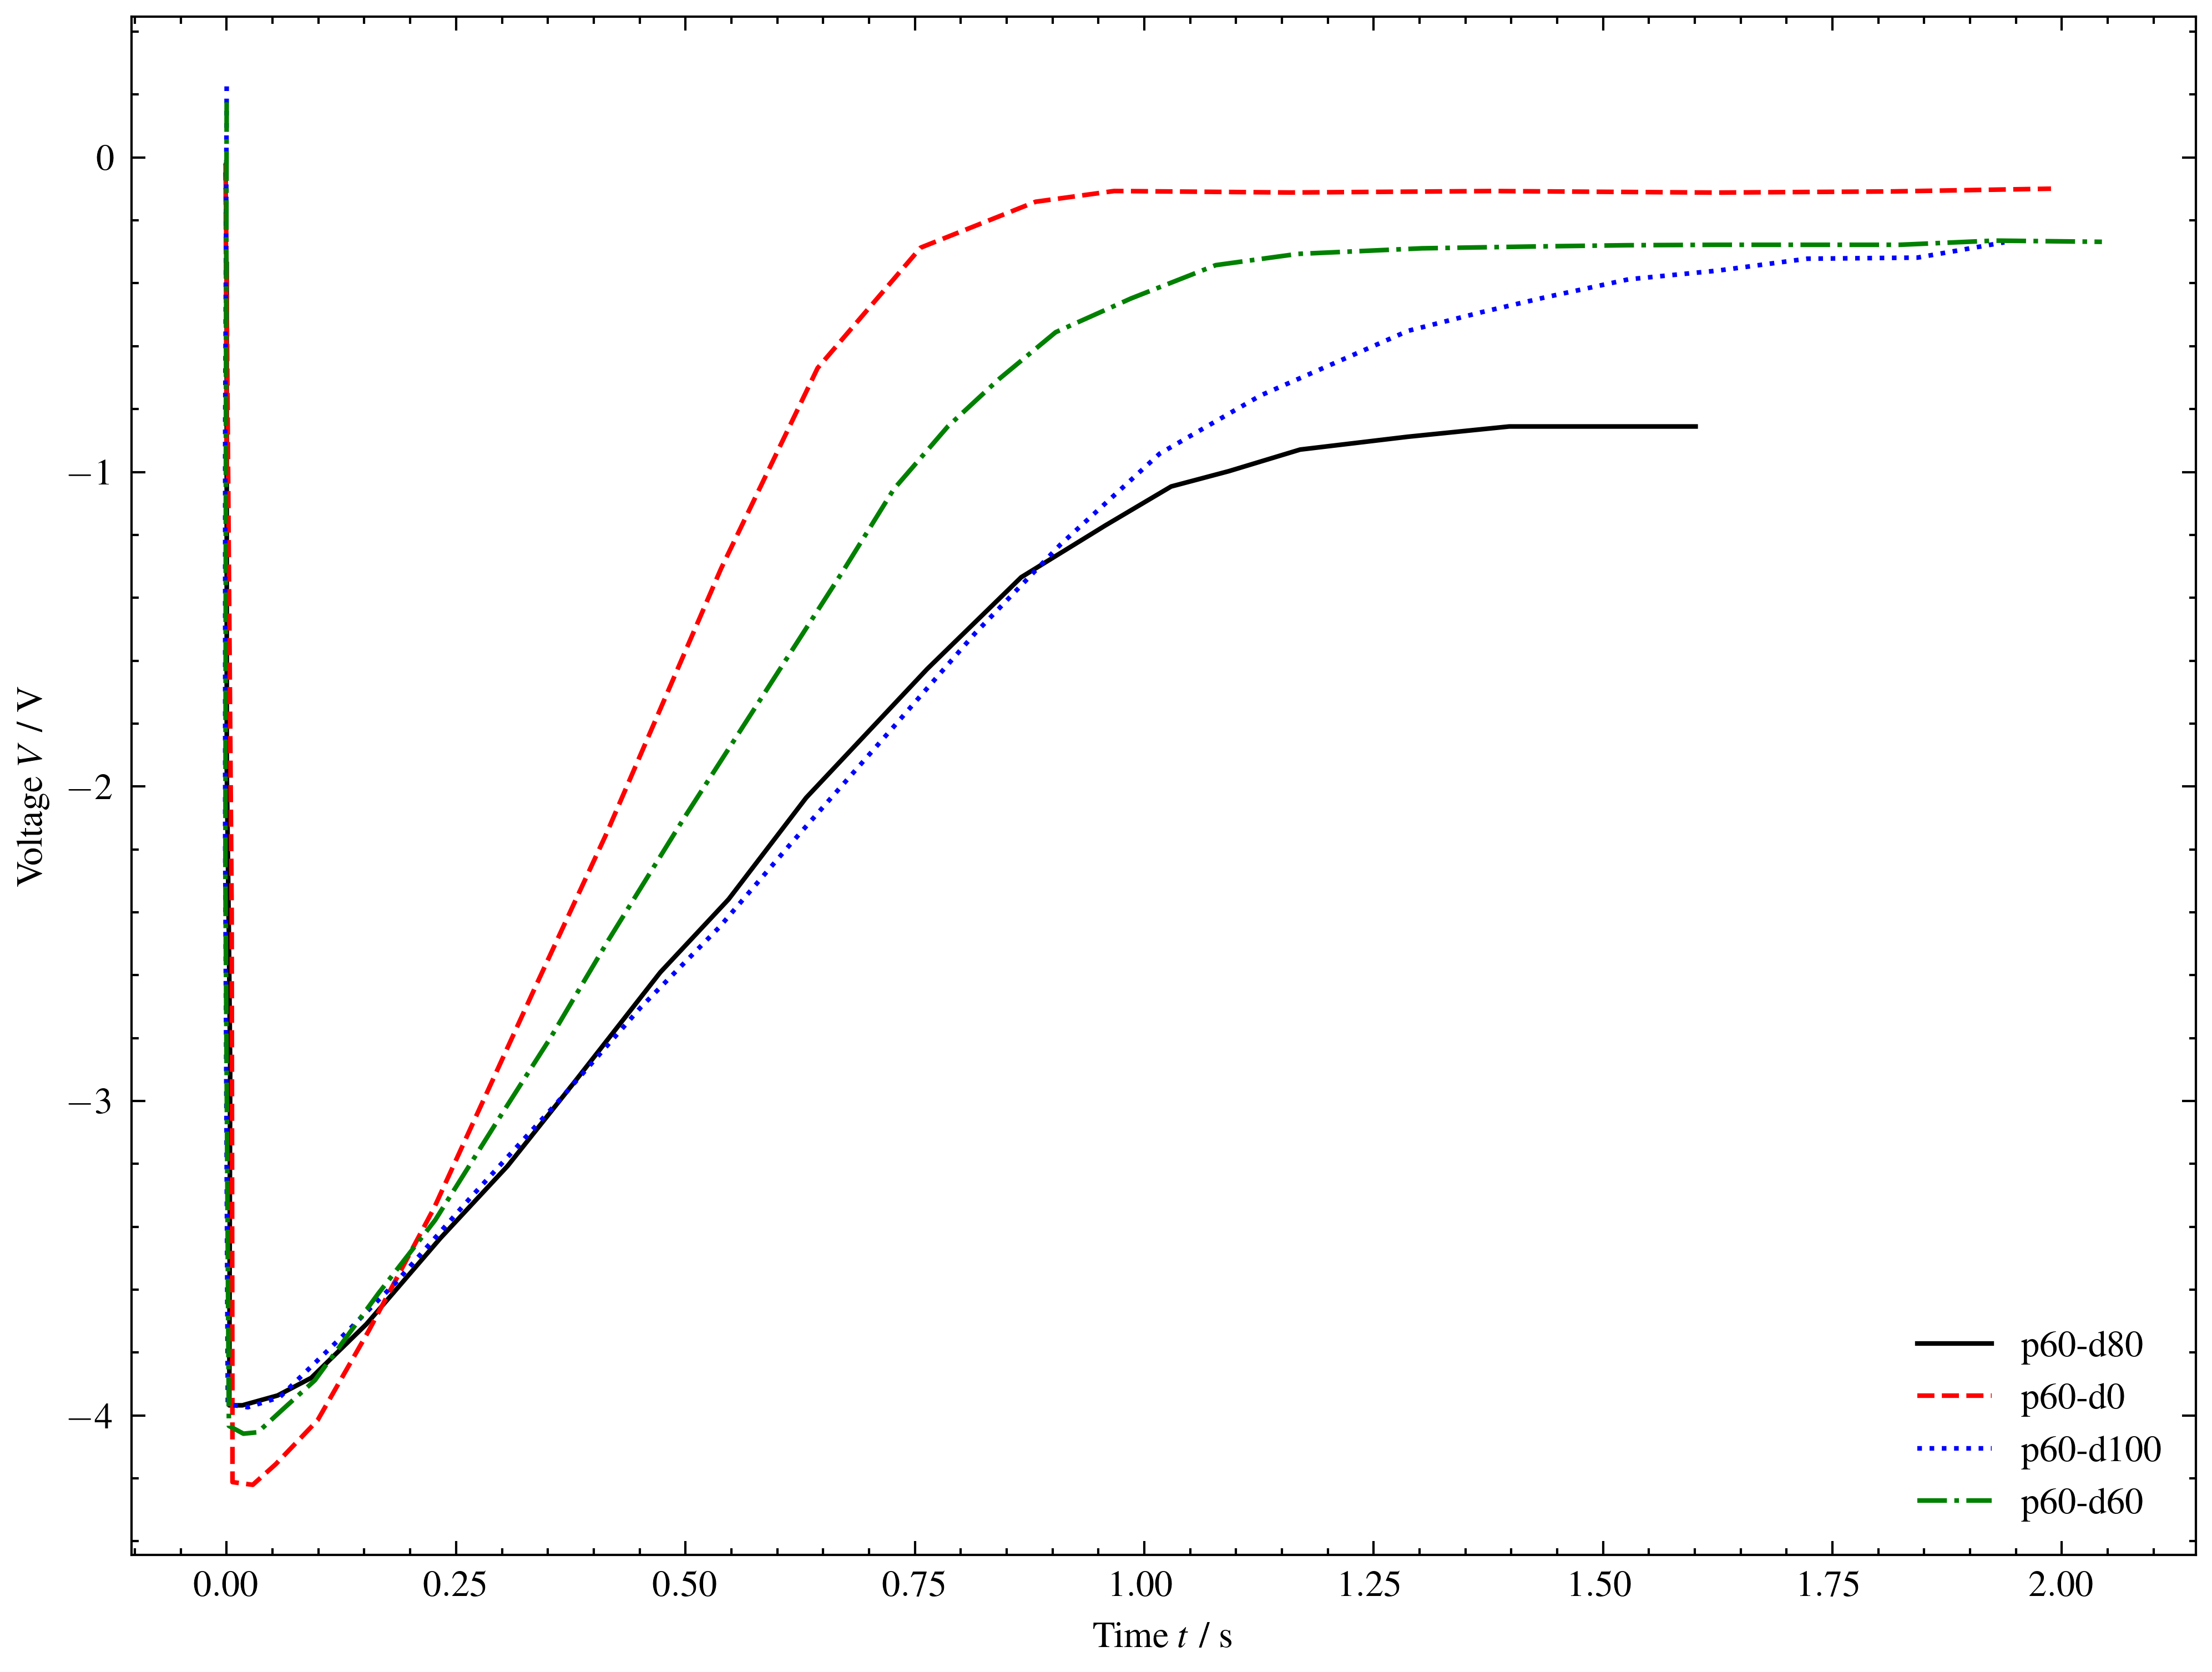
\includegraphics[width=0.8\linewidth]{src/figures/oscilloscope-grouped/p-60.png}
		\subcaption{$P = 60$}
	\end{subfigure}
	\begin{subfigure}{0.48\columnwidth}
		\centering
		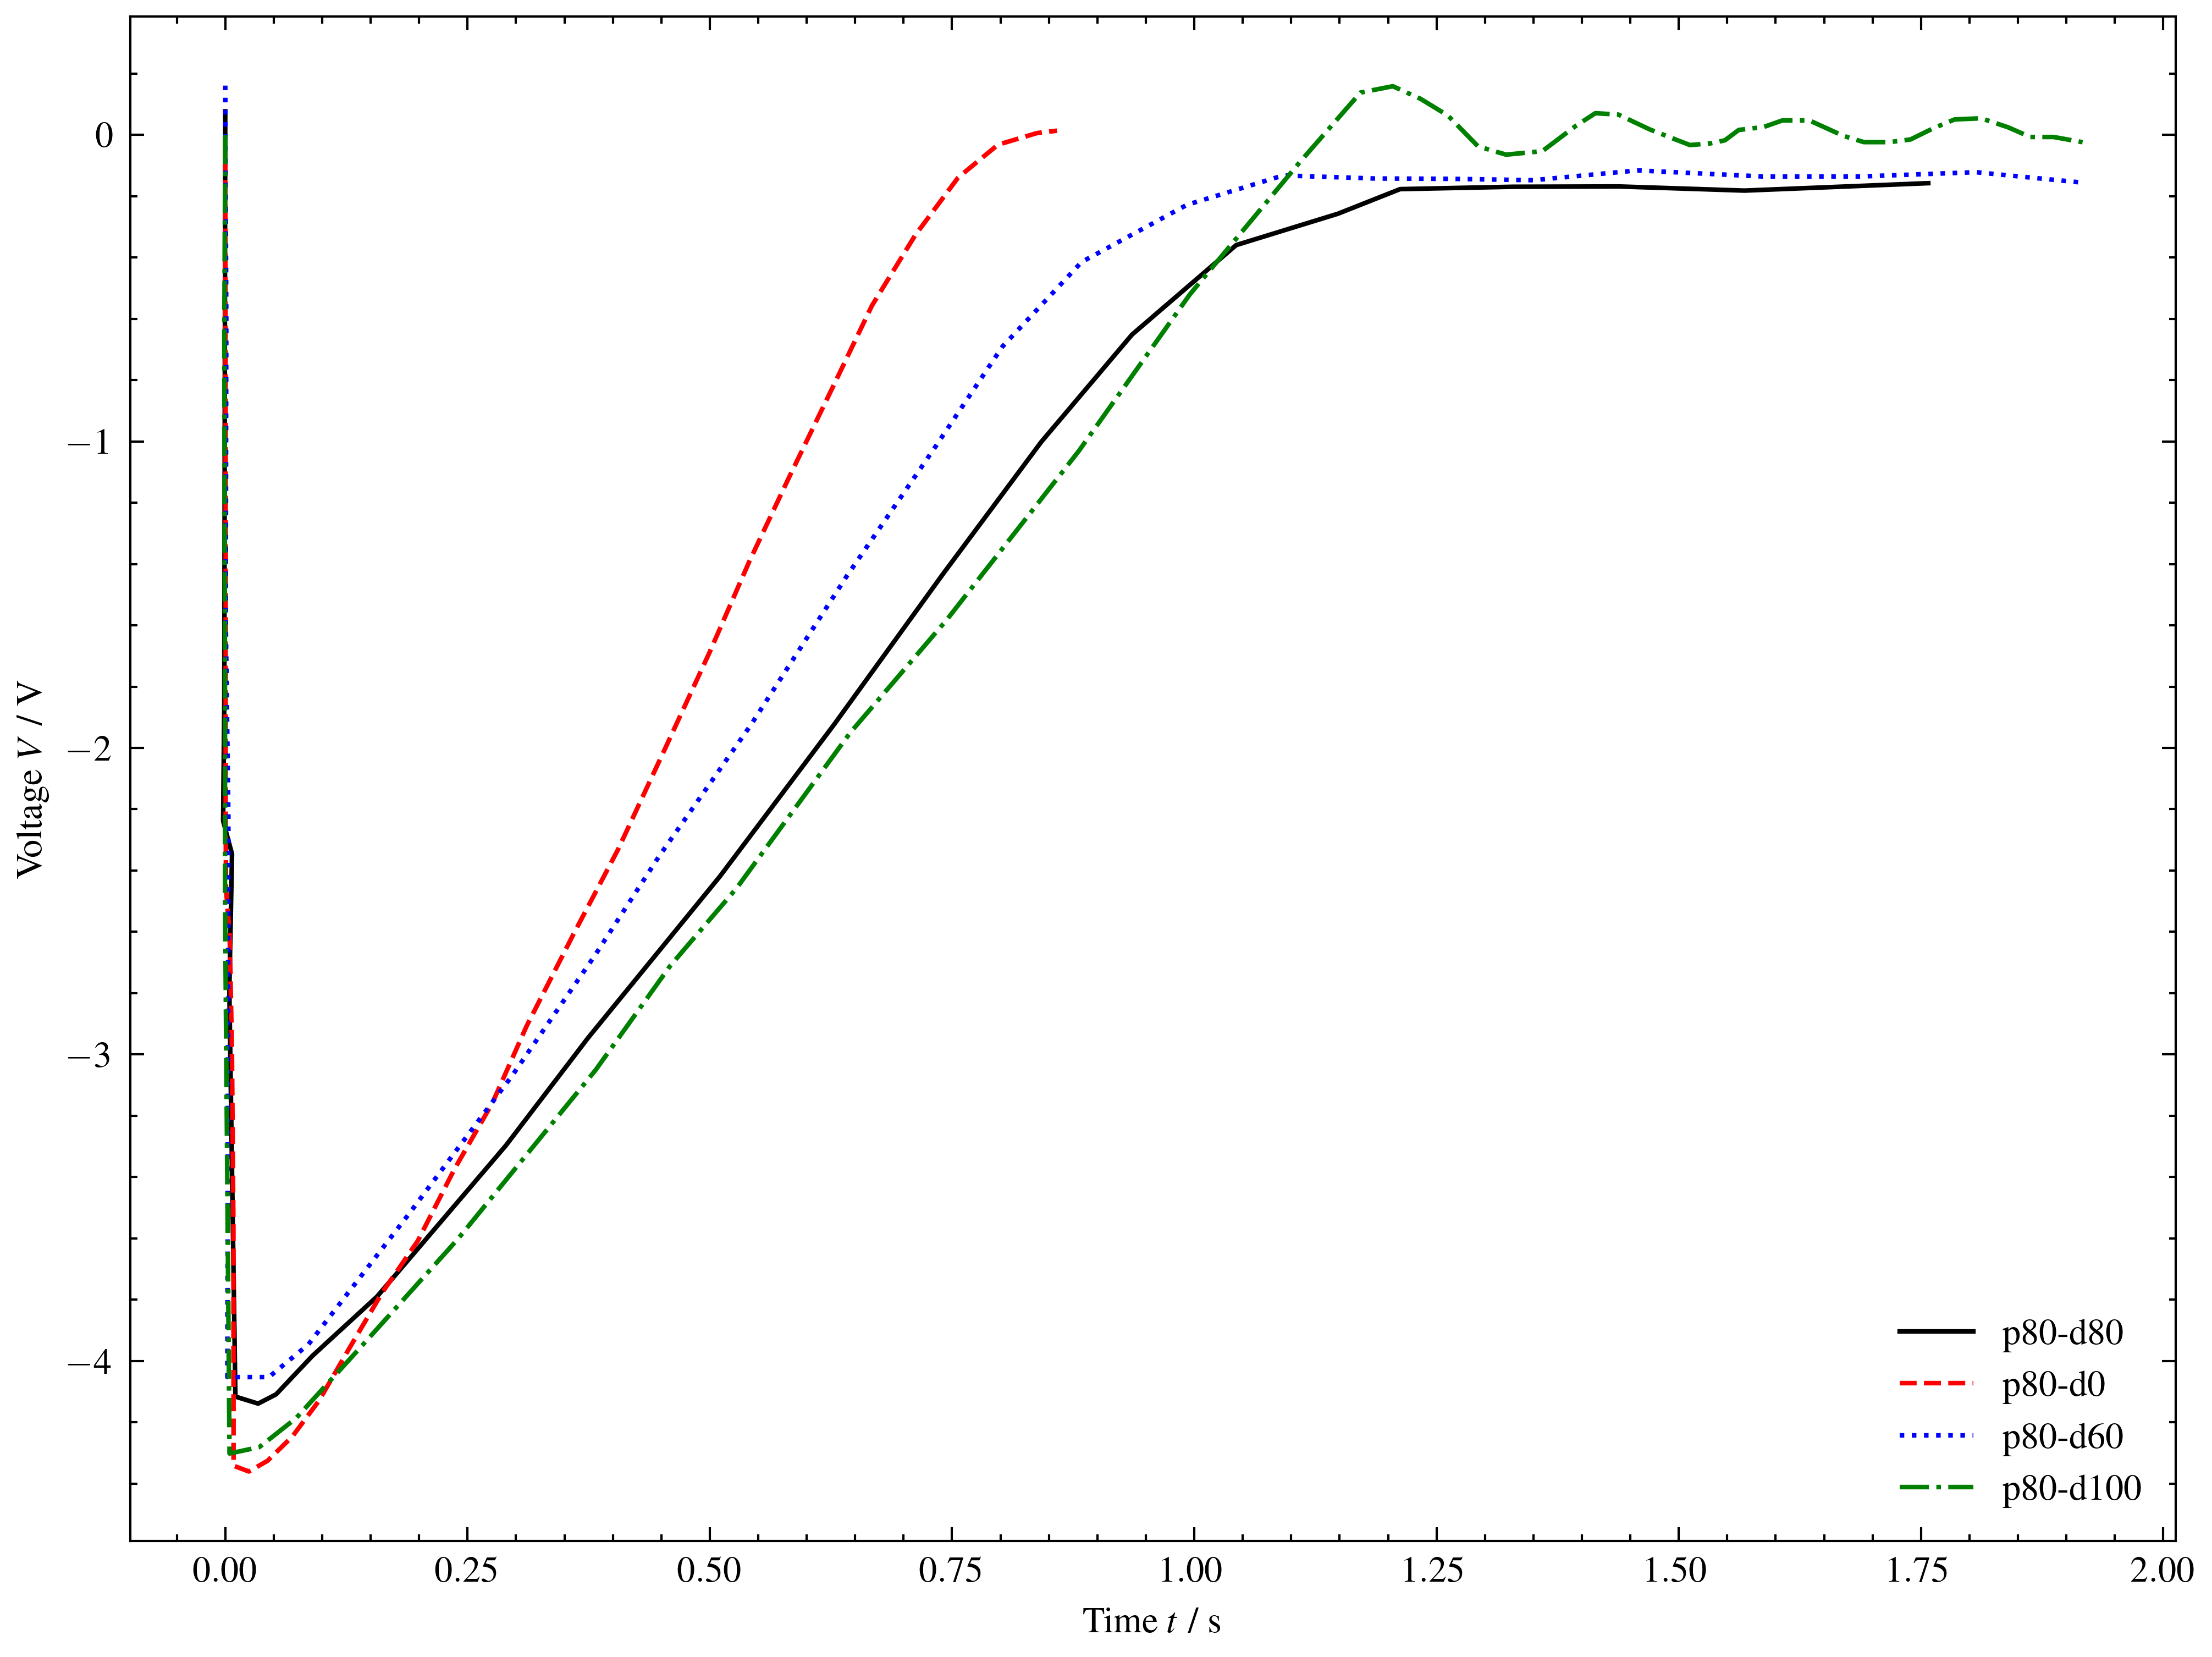
\includegraphics[width=0.8\linewidth]{src/figures/oscilloscope-grouped/p-80.png}
		\subcaption{$P = 80$}
	\end{subfigure}
	\begin{subfigure}{0.48\columnwidth}
		\centering
		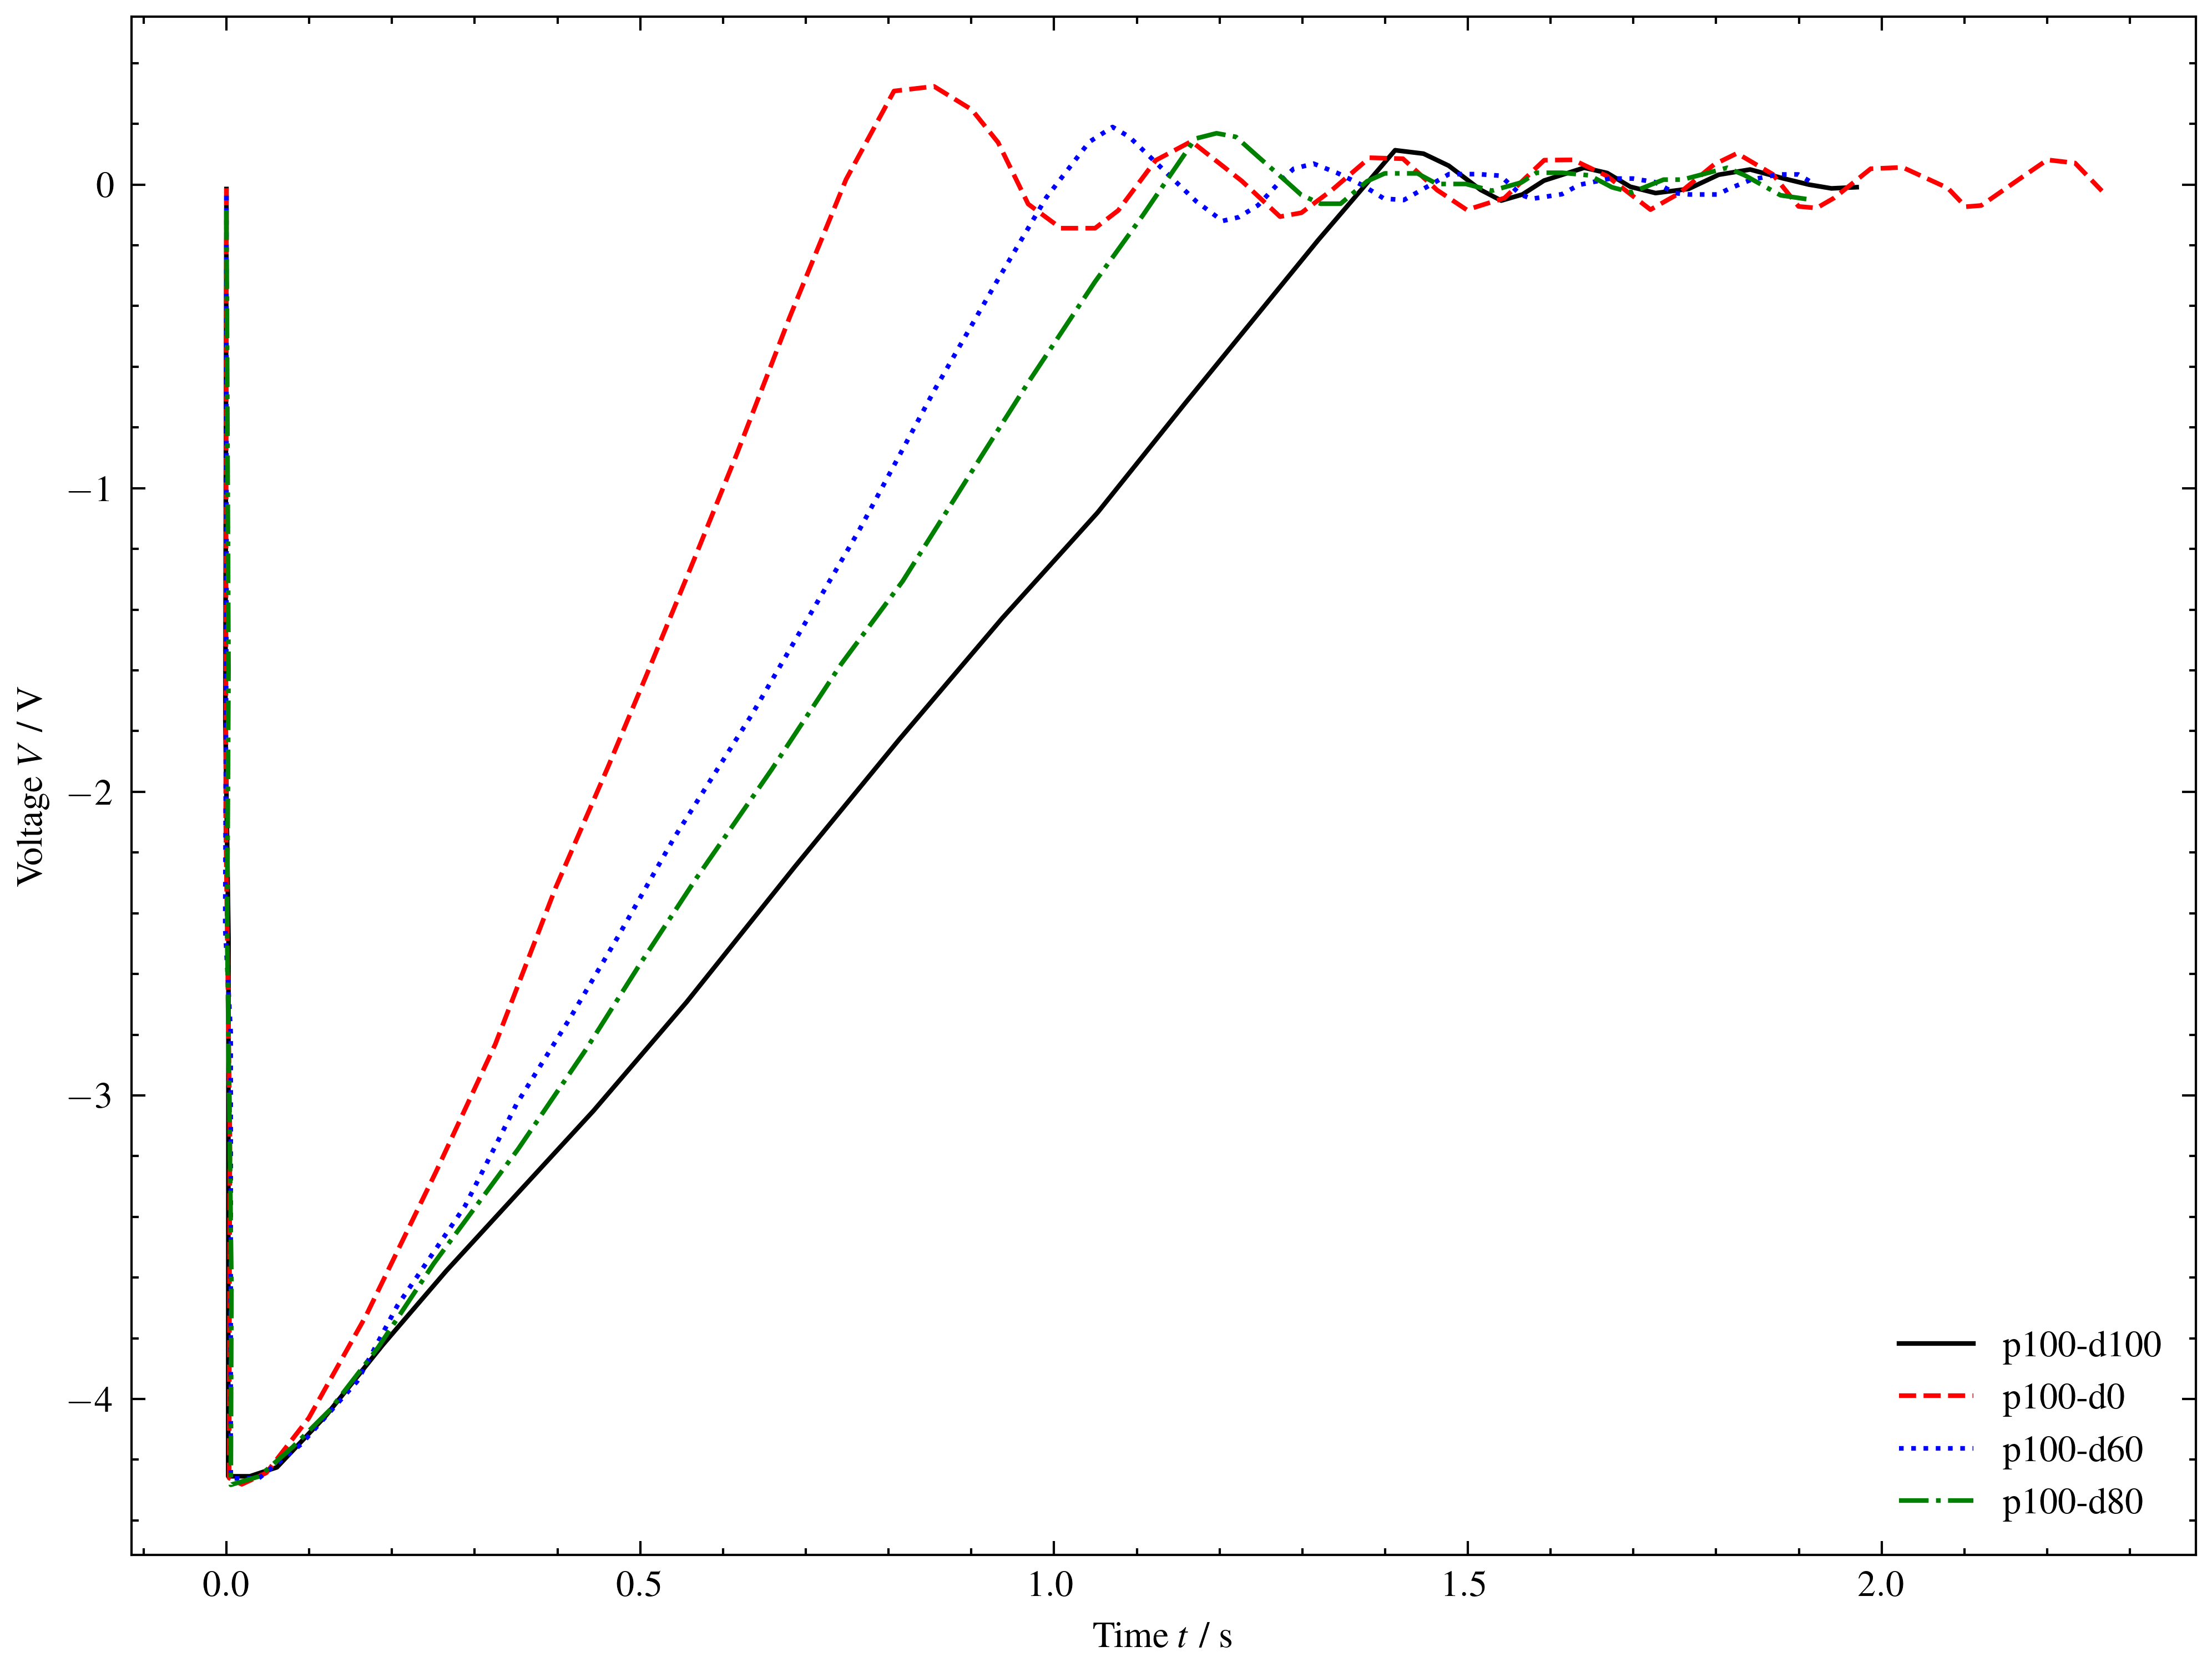
\includegraphics[width=0.8\linewidth]{src/figures/oscilloscope-grouped/p-100.png}
		\subcaption{$P = 100$}
	\end{subfigure}
	\caption{ある$P$に対する$D$を変化させたときの波形}\label{fig:oscilloscope-grouped-p}
\end{figure}


図\ref{fig:oscilloscope-grouped-d}から、
ある$D$に対して、$P=60$、$P=80$、$P=100$と大きくなるにつれオーバーシュートが発生し、
オーバーシュート量も大きくなっている。
これは、2次遅れ系の式\ref{eq:characteristic-function}または\ref{eq:characteristic-function2}で表される
分母多項式はともに$s^2+2\zeta\omega s+\omega^2$であり、
極は$s=-\zeta\omega \pm \omega \sqrt{\zeta^2-1}$なる。
したがって、$\zeta\geq1$のとき2次遅れ系の極は実数で振動せず0に収束している一方で、
$\zeta<1$のときは2次遅れ系の極が虚数となり逆ラプラス変換したときに減衰振動となるため、
オーバーシュートが発生していると考えられる。
実際、表\ref{tab:zeta}からもわかる様に、
$\zeta<1$のときである、
$(P, D) = (80, 0), (100, 0), (100, 60), (100, 80), (100, 100)$
のときにオーバーシュートが発生している。
また、図\ref{fig:oscilloscope-grouped-p}から、
ある$P$に対して$D$を大きくすると、
上記のようにオーバーシュート量が小さくなる一方で速応性が下がり遅れるとわかる。


伝達関数が\ref{eq:characteristic-function}、\ref{eq:characteristic-function2}式で表されるとき、
$\zeta=0.2, 0.5, 1.0, 1.5, 2.0$に対して、$\omega=5, 6, 25$として変化させ、
ボード線図とステップ応答をシミュレーションしたものを次に示す。
\footnote{
	シミュレーションに使用したコードは\url{https://github.com/shunta0213/b3-e1-exp/tree/main/src/scripts}にある。
}
図\ref{fig:bode-phase-step-ideal-group-omega}は$\omega$ごとにまとめたもの、
図\ref{fig:bode-phase-step-ideal-group-real}は$D$が一定となるような$\omega$、$\zeta$の組についてまとめたものである。
この理想的なステップ応答と実験の結果を比較すると、
$\omega$一定で$\zeta$が大きくなる、すなわち$P$一定で$D$を大きくすると
オーバーシュート量が小さくなり、速応性が下がるという点で整合している。
一方で、$D$一定として$P$を変化させたときは、
図\ref{fig:bode-phase-step-ideal-group-real}から$P$を大きくすると
速応性が上がるはずであるが、
図\ref{fig:oscilloscope-grouped-d}では$P$を大きくしても速応性が上がっていない。


\begin{figure}
	\centering
	\begin{subfigure}{0.8\linewidth}
		\centering
		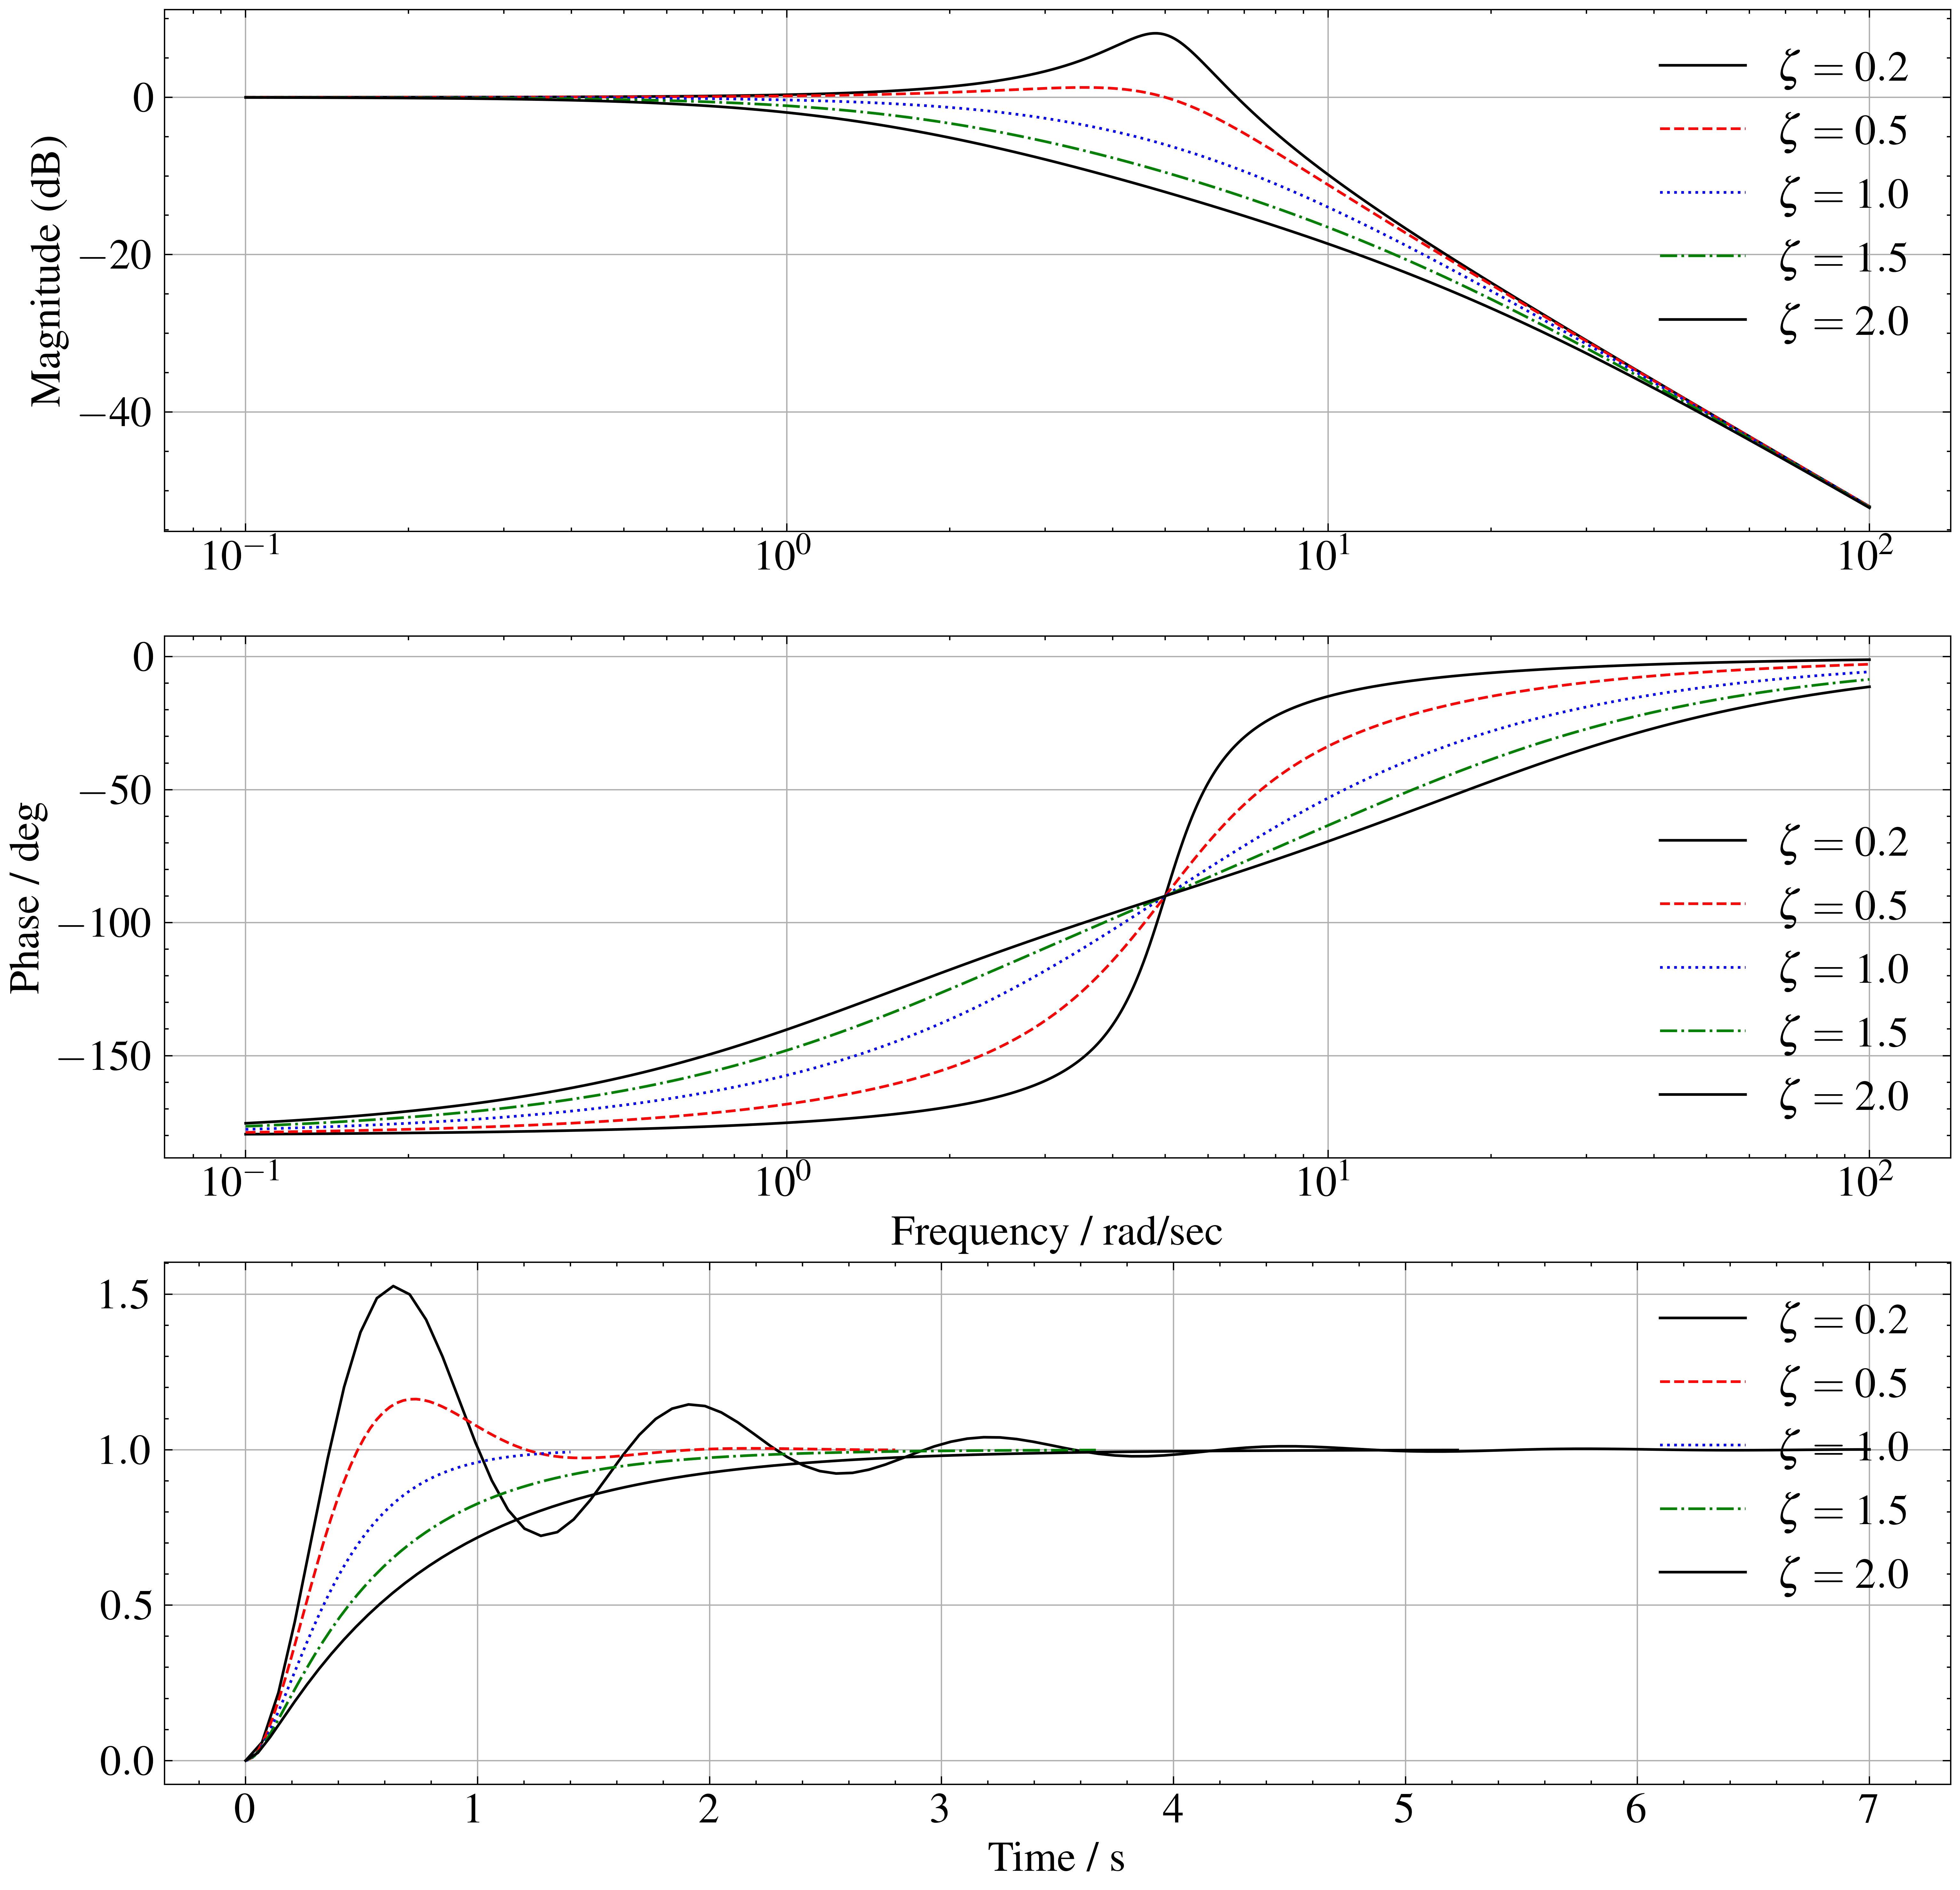
\includegraphics[width=0.8\linewidth]{src/figures/bode-phase-step-ideal-group-omega/bode-phase-step-ideal-group-omega-5.png}
		\subcaption{$\omega = 5$}\label{fig:bode-phase-step-ideal-group-omega-5}
	\end{subfigure}
	\begin{subfigure}{0.8\linewidth}
		\centering
		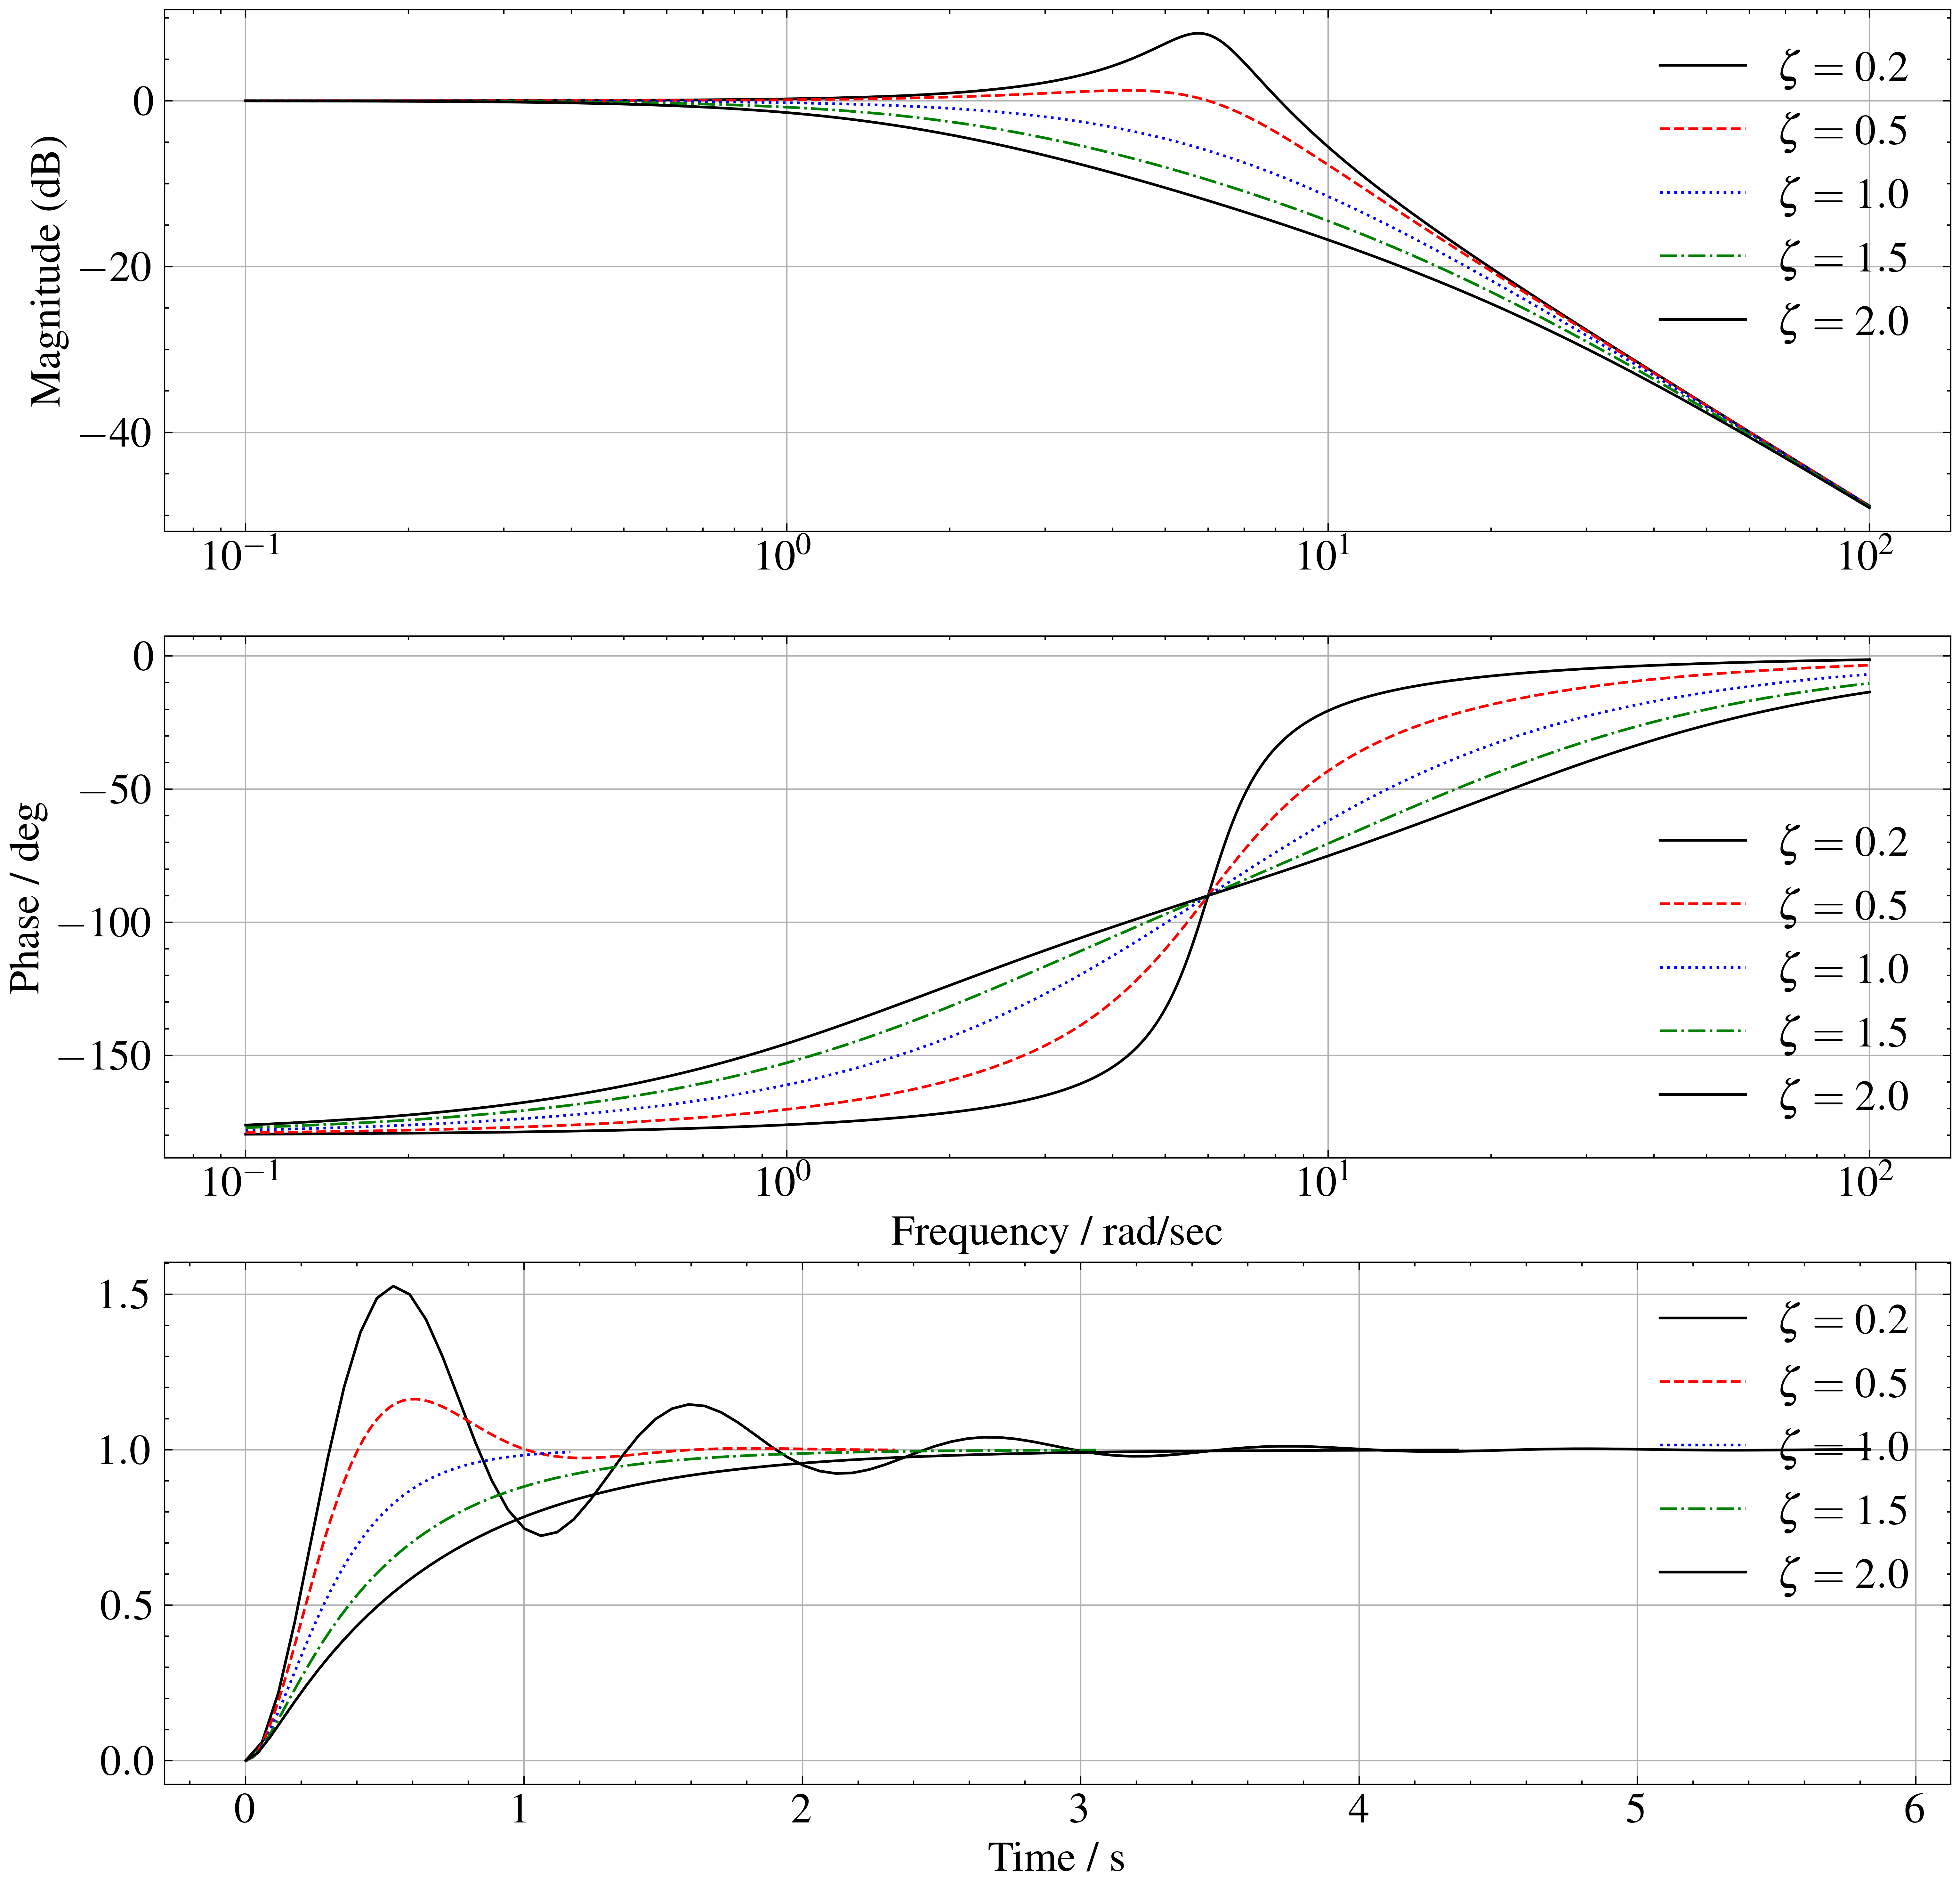
\includegraphics[width=0.8\linewidth]{src/figures/bode-phase-step-ideal-group-omega/bode-phase-step-ideal-group-omega-6.png}
		\subcaption{$\omega = 6$}\label{fig:bode-phase-step-ideal-group-omega-6}
	\end{subfigure}
	\caption{ある$\omega$に対して、$\zeta$を変化させたときのボード線図とステップ応答}\label{fig:bode-phase-step-ideal-group-omega}
\end{figure}


\begin{figure}
	\centering
	\addtocontents{figure}{-1}
	\begin{subfigure}{0.8\linewidth}
		\setcounter{subfigure}{2}
		\centering
		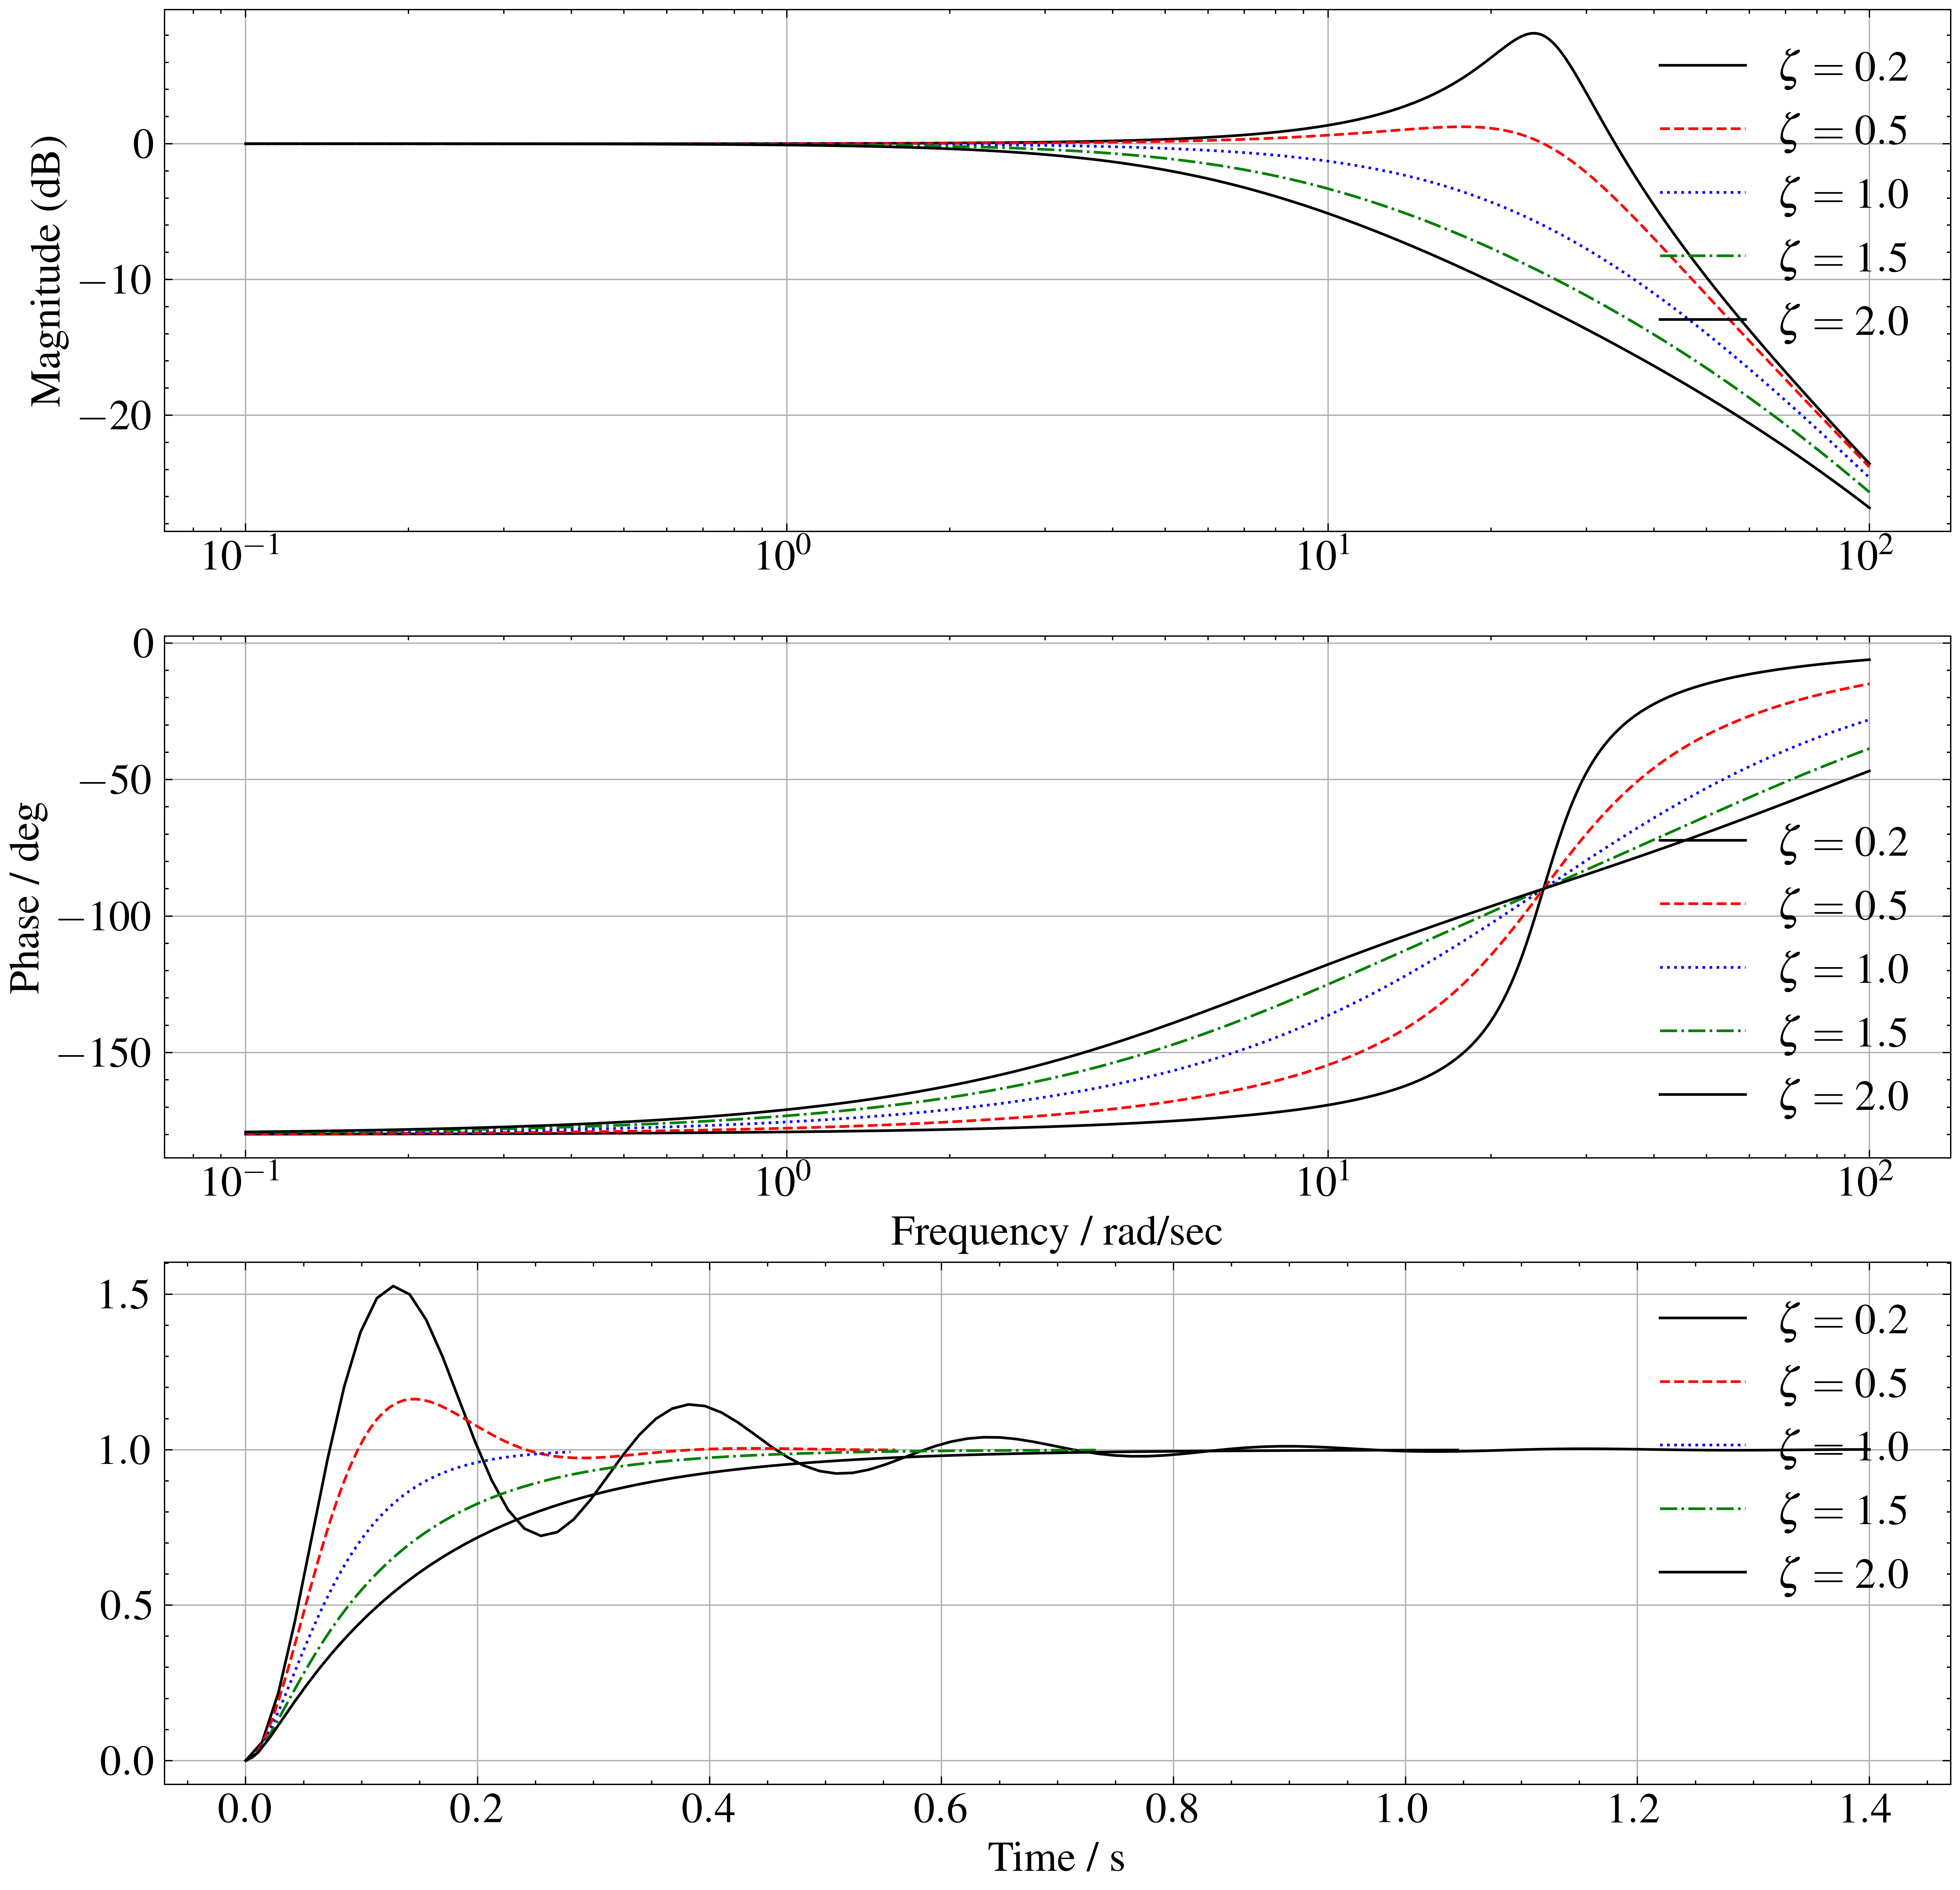
\includegraphics[width=0.8\linewidth]{src/figures/bode-phase-step-ideal-group-omega/bode-phase-step-ideal-group-omega-25.png}
		\subcaption{$\omega = 25$}\label{fig:bode-phase-step-ideal-group-omega-25}
	\end{subfigure}
	\caption{ある$\omega$に対して、$\zeta$を変化させたときのボード線図とステップ応答(続き)}
\end{figure}

\begin{figure}
    \centering
    \begin{subfigure}{0.8\linewidth}
        \centering
        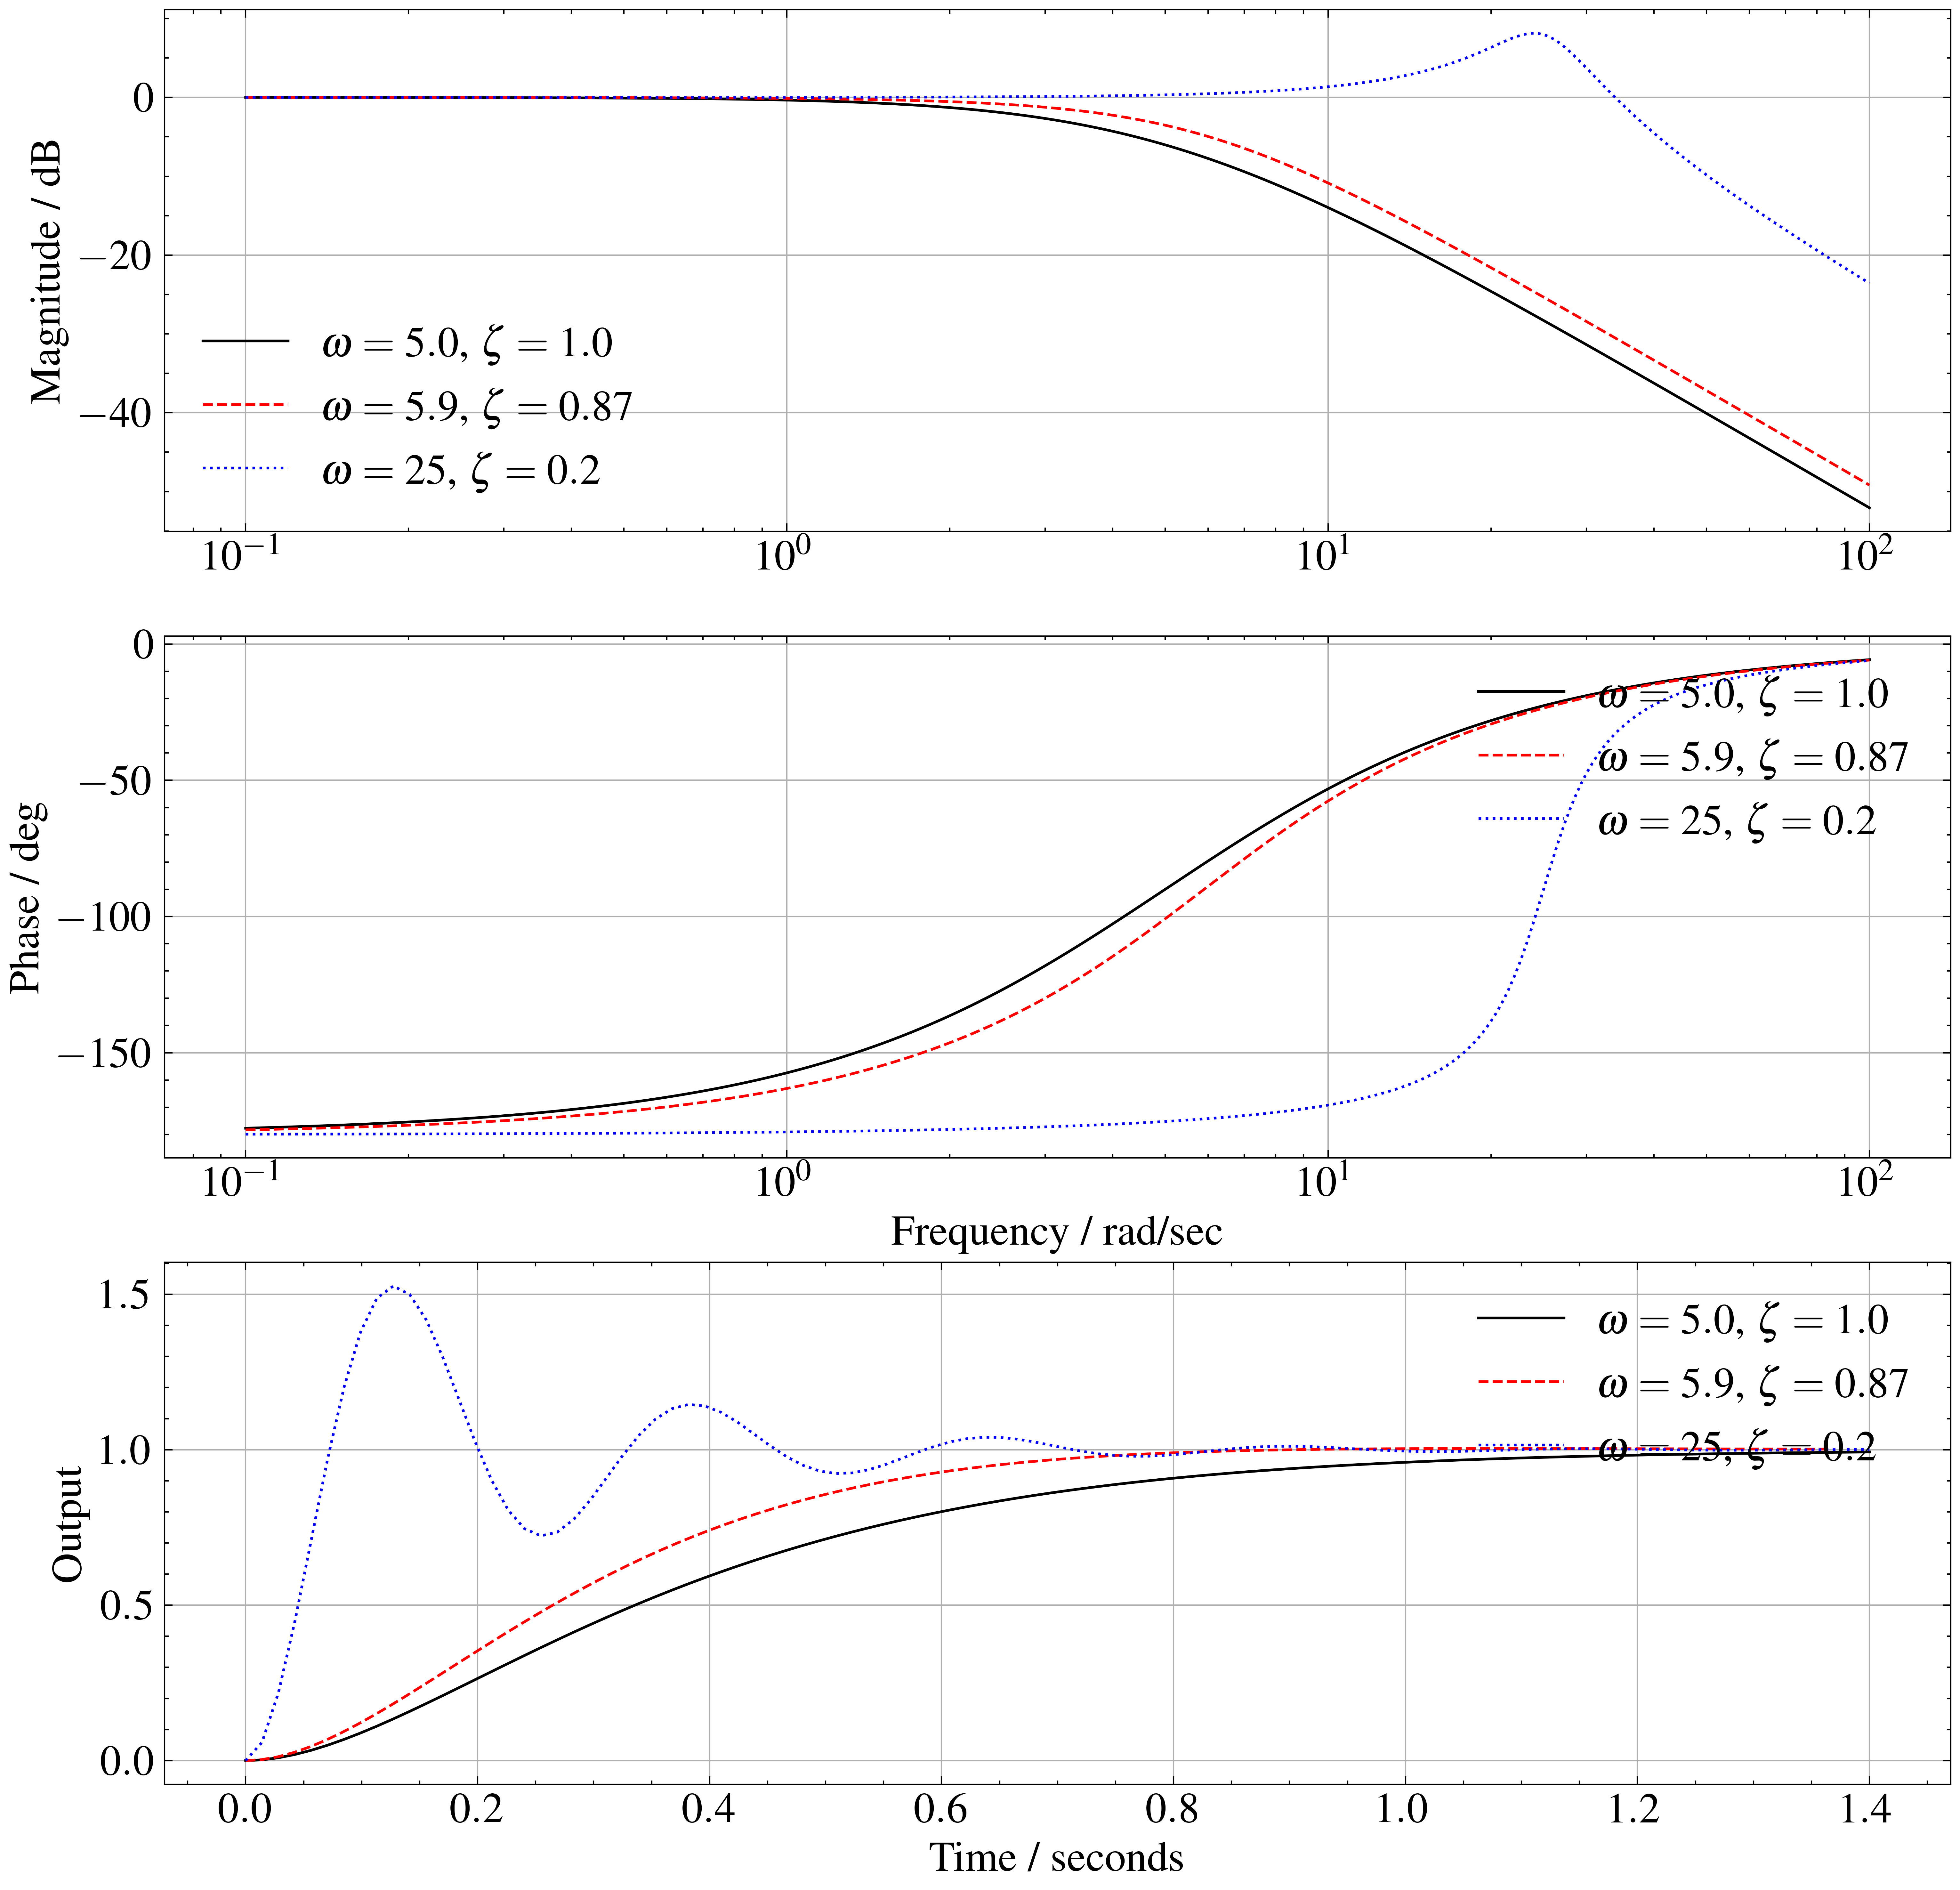
\includegraphics[width=0.8\linewidth]{src/figures/bode-phase-step-ideal-group-real/bode-phase-step-ideal-group-real-1.png}
        \subcaption{$D = 0$のときの$\zeta$、$\omega$の近侍値に対するボード線図とステップ応答}\label{fig:bode-phase-step-ideal-group-real-d-0}
    \end{subfigure}
    \begin{subfigure}{0.8\linewidth}
        \centering
        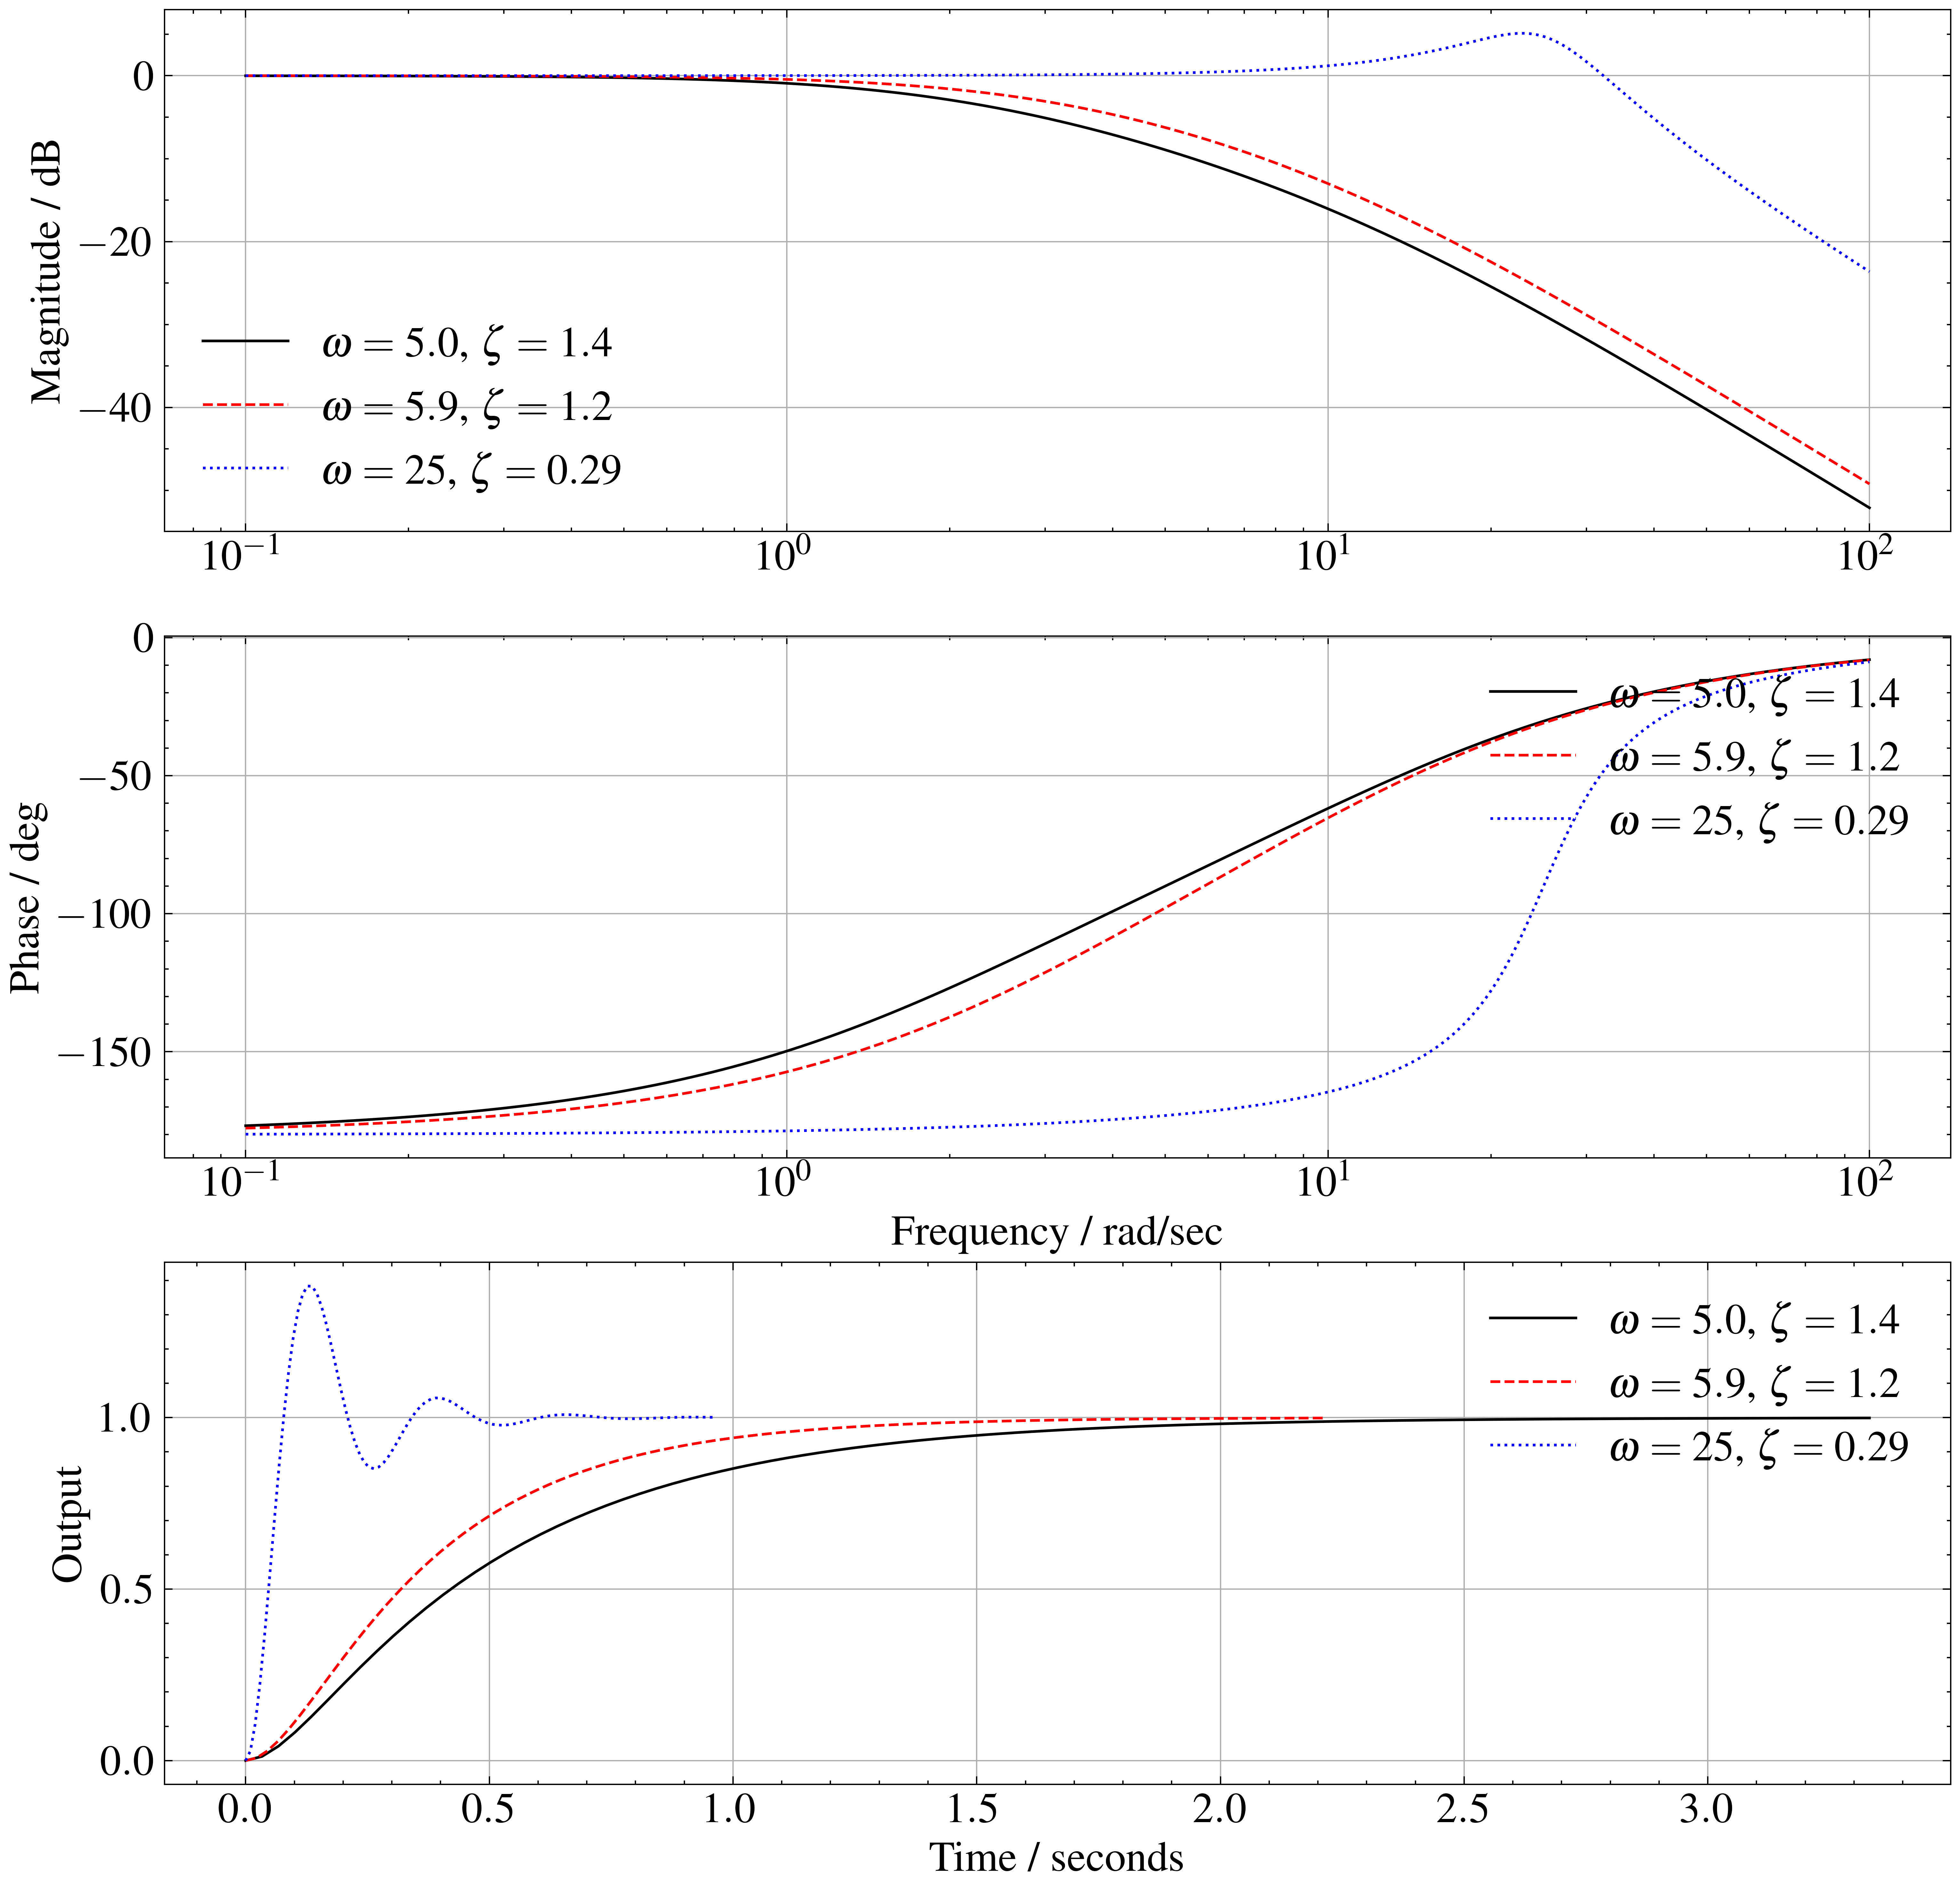
\includegraphics[width=0.8\linewidth]{src/figures/bode-phase-step-ideal-group-real/bode-phase-step-ideal-group-real-2.png}
        \subcaption{$D = 60$のときの$\zeta$、$\omega$の近侍値に対するボード線図とステップ応答}\label{fig:bode-phase-step-ideal-group-real-d-60}
    \end{subfigure}
    \caption{ある$D$に対して、$P$を変化させたときのボード線図とステップ応答}\label{fig:bode-phase-step-ideal-group-real}
\end{figure}


\begin{figure}
    \addtocounter{figure}{-1}
    \centering
    \begin{subfigure}{0.8\linewidth}
        \setcounter{subfigure}{2}
        \centering
        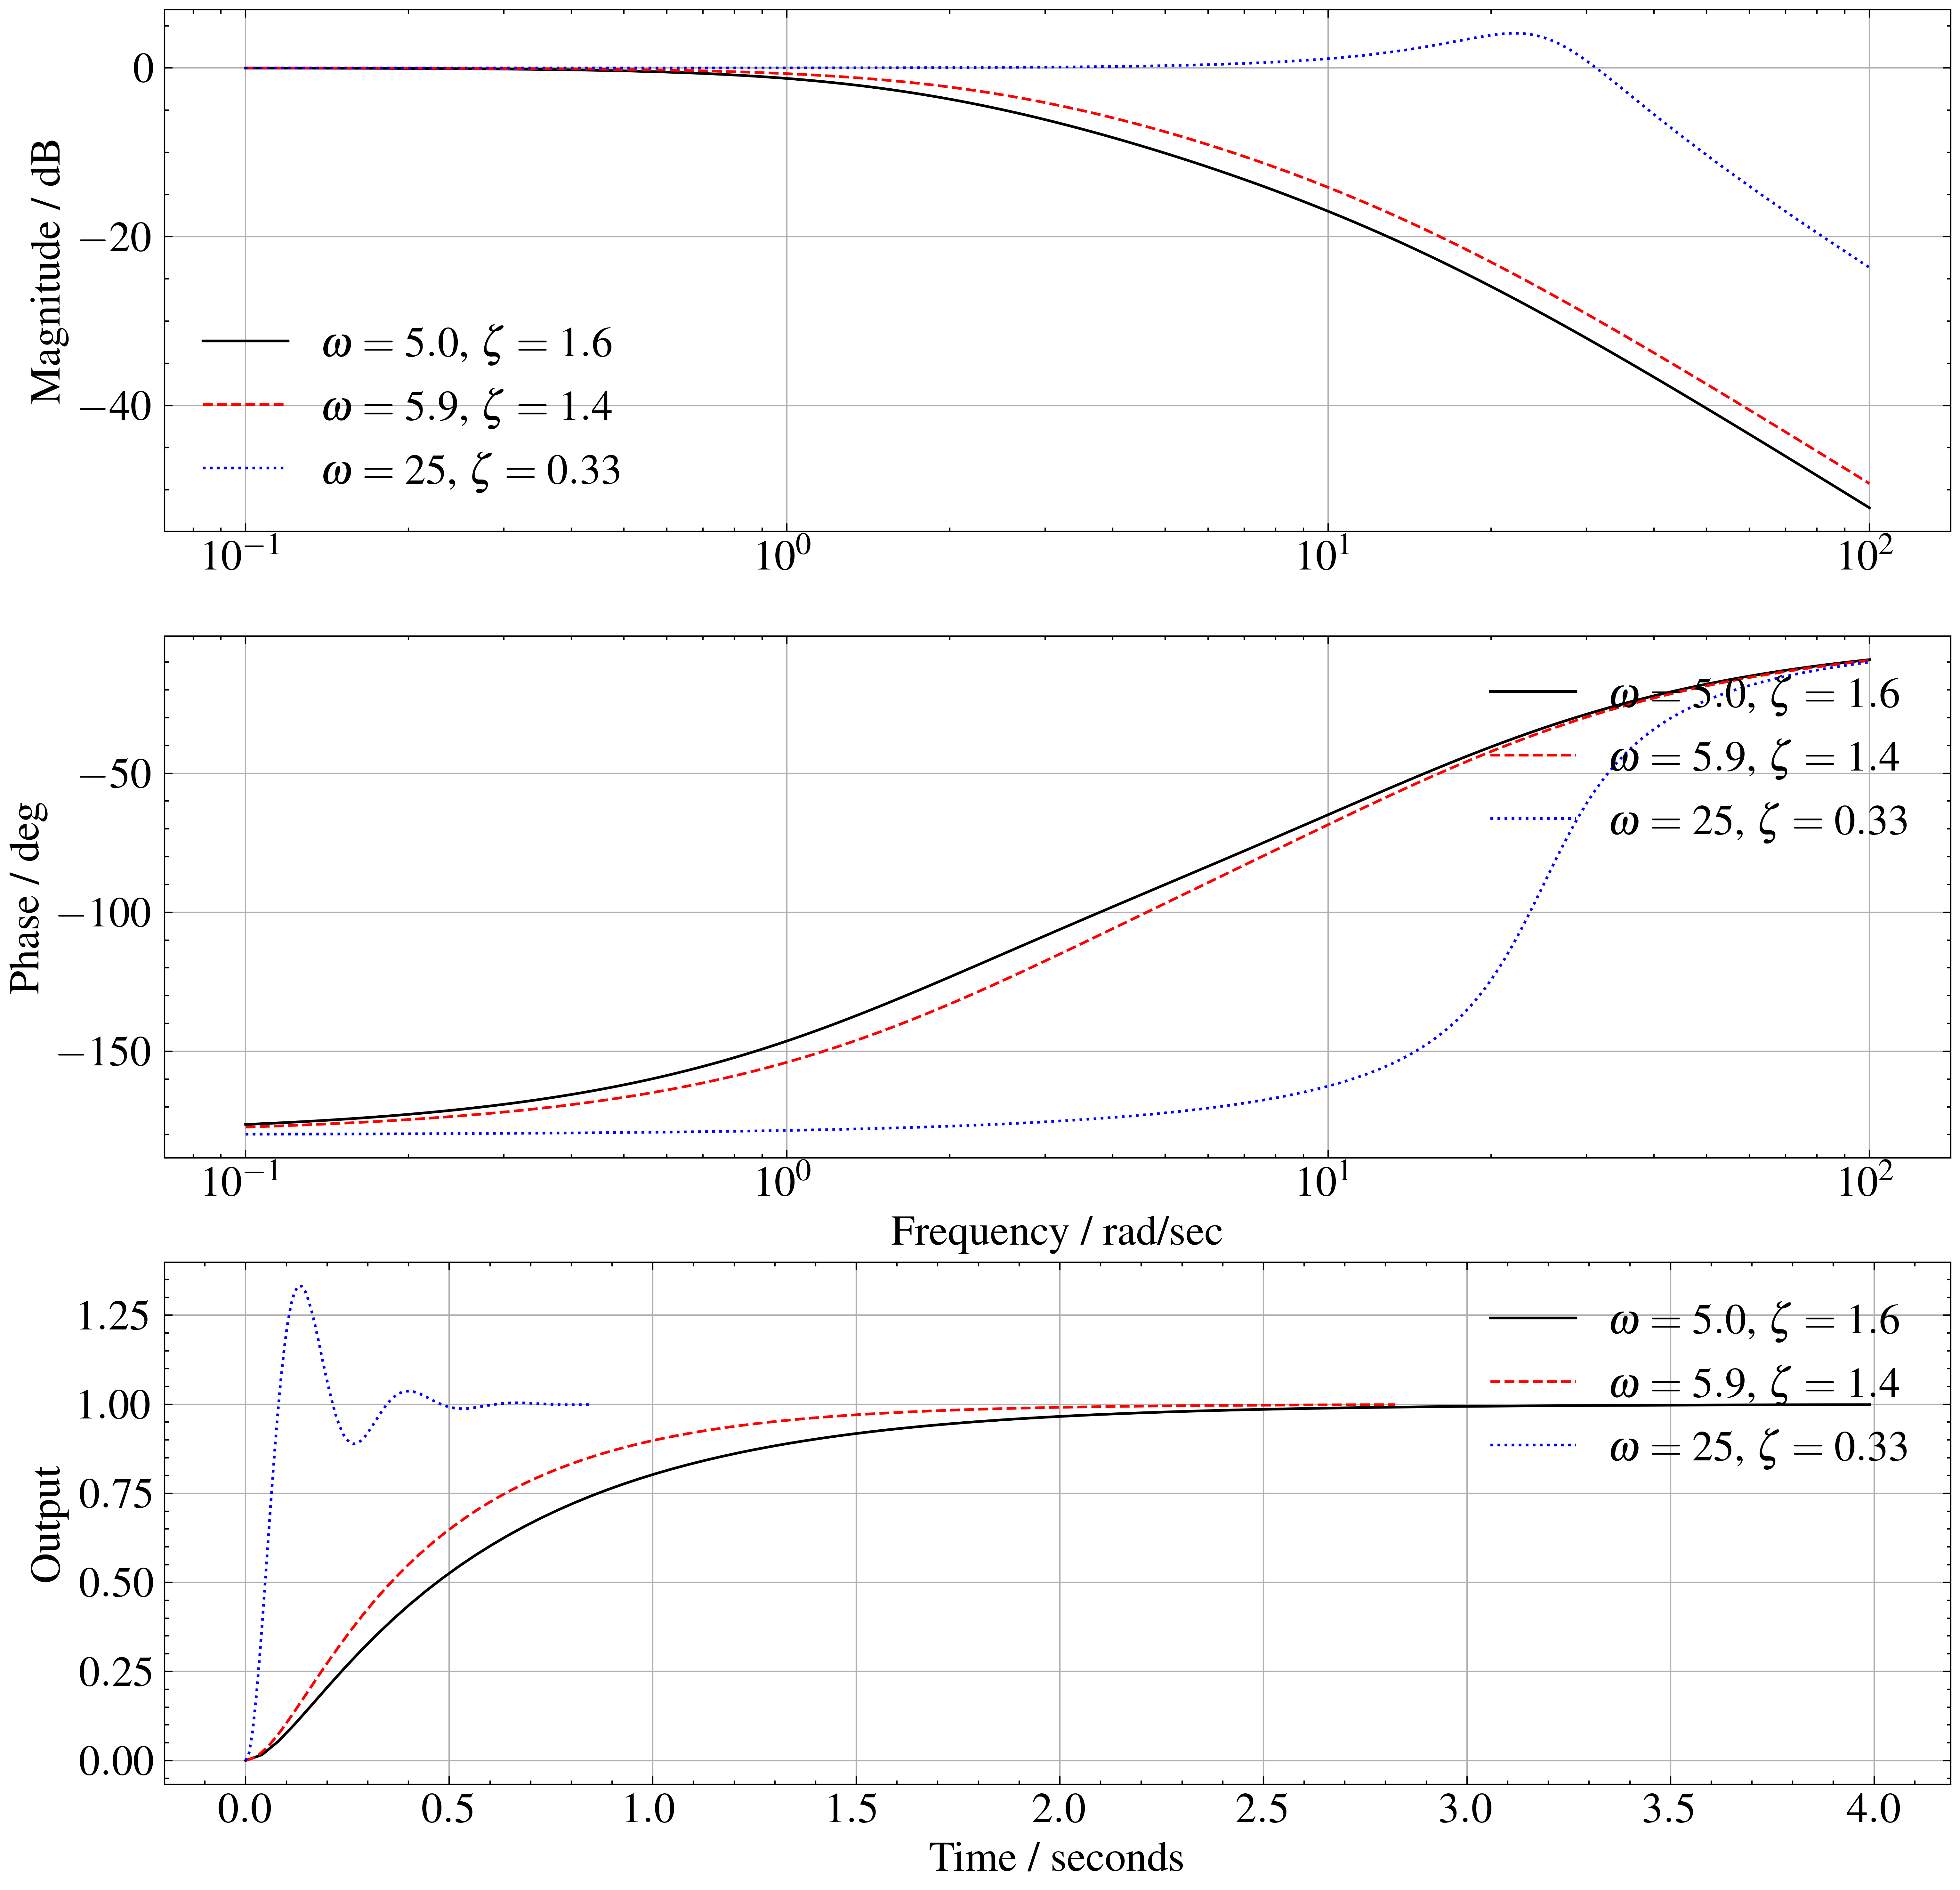
\includegraphics[width=0.8\linewidth]{src/figures/bode-phase-step-ideal-group-real/bode-phase-step-ideal-group-real-3.png}
        \subcaption{$D = 80$のときの$\zeta$、$\omega$の近侍値に対するボード線図とステップ応答}\label{fig:bode-phase-step-ideal-group-real-d-80}
    \end{subfigure}
    \begin{subfigure}{0.8\linewidth}
        \centering
        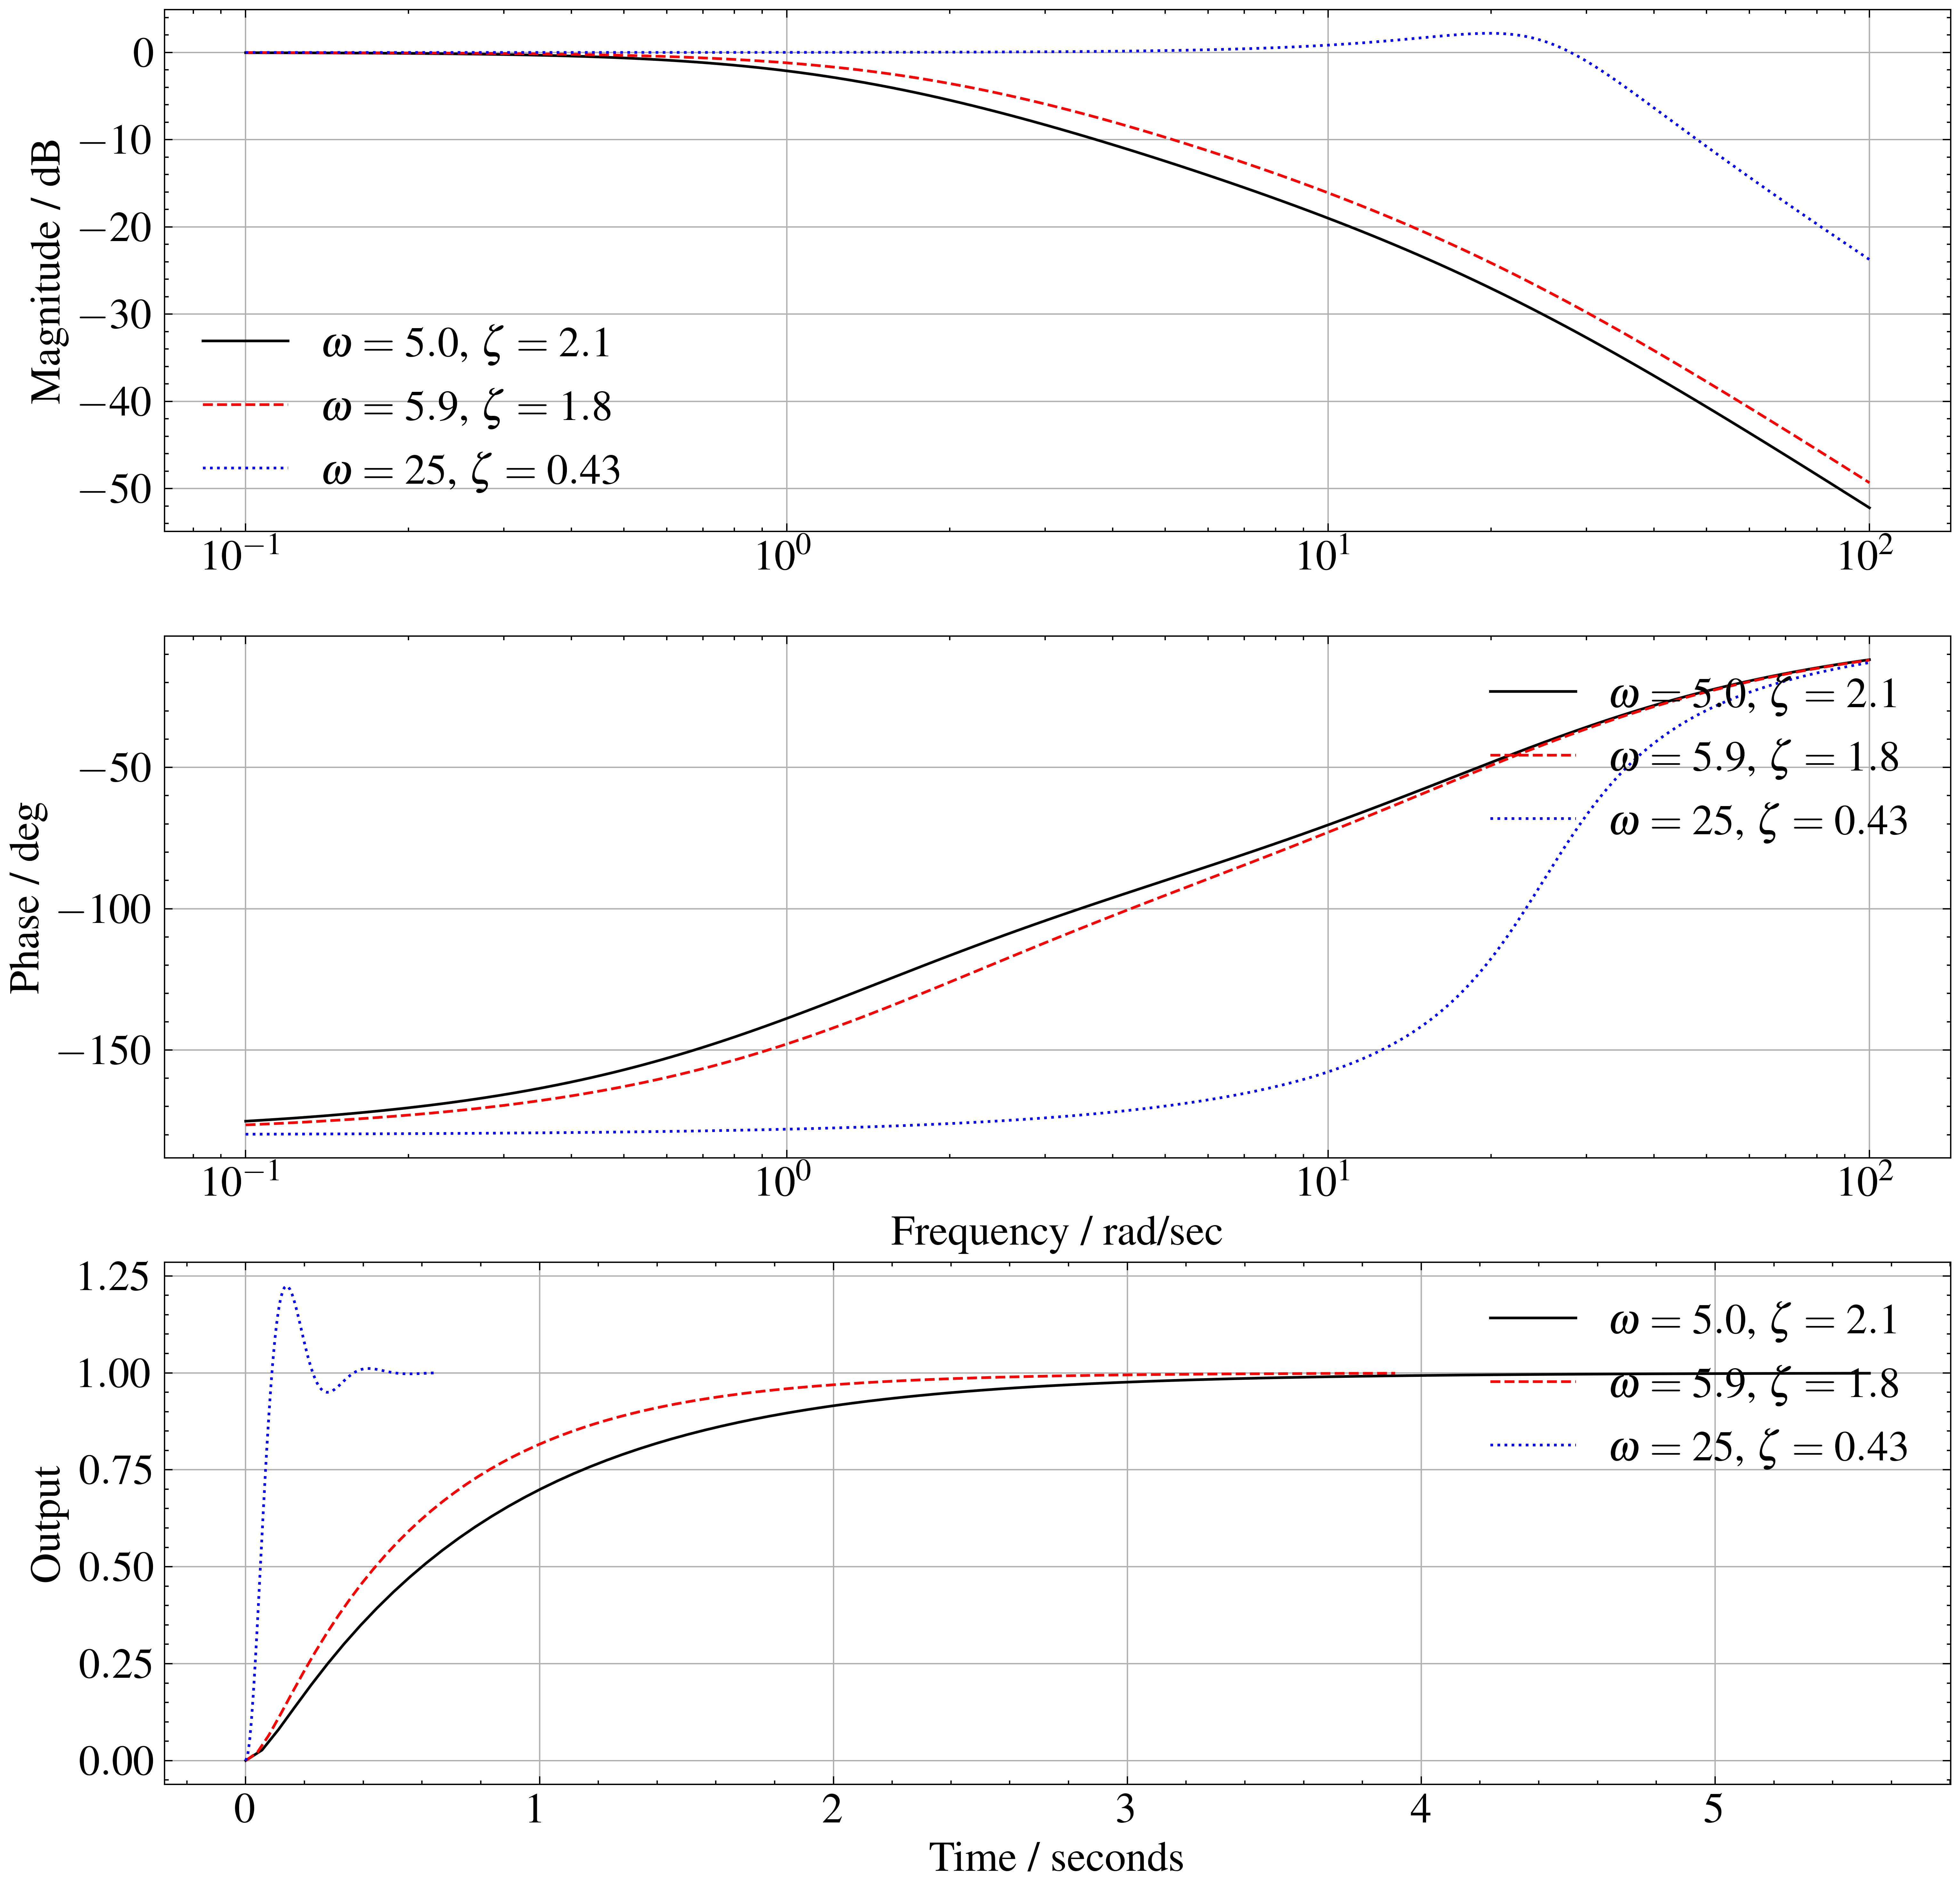
\includegraphics[width=0.8\linewidth]{src/figures/bode-phase-step-ideal-group-real/bode-phase-step-ideal-group-real-4.png}
        \subcaption{$D = 100$のときの$\zeta$、$\omega$の近侍値に対するボード線図とステップ応答}\label{fig:bode-phase-step-ideal-group-real-d-100}
    \end{subfigure}
    \caption{ある$D$に対して、$P$を変化させたときのボード線図とステップ応答(続き)}
\end{figure}


\end{document}
